% Chapter 4
\label{Capítulo4}
\chapter{Implementação}
\begin{center}
	\textit{``Do or do not. There is no try.''}

	Master Yoda
\end{center}
Neste capítulo aborda-se com mais pormenor os aspectos mais técnicos do \acrshort{lare}, tendo como base a arquitectura apresentada na Figura \ref{fig:arquitecturalore}.

O desenvolvimento começou pela implementação e desenvolvimento do servidor \textit{Flask} e página \textit{web}. O primeiro circuito a ser testado e integrado foi a Lei de Ohm. O projecto foi evoluindo com a adição dos restantes circuitos que compõem o \acrshort{lare}.

O \acrshort{ide} utilizado no desenvolvimento do \textit{software} foi o \textit{Visual Studio Code}\footnote{\url{https://code.visualstudio.com/}} e o projecto está alojado no \textit{GitHub}. O sistema operativo instalado no RaspberryPI 5 foi uma versão ligeiramente modificada do \textit{Arch Linux ARM}.

Os circuitos que compõem o \acrshort{lare} foram testados e validados individualmente em placas brancas, antes de se proceder à construção da matriz de placas, como referido na Secção \ref{sec:matriz}.

\section{Hardware}
\subsection{Relés}
\label{sec:hwreles}

\textbf{---Já foi referido com pormenor no cap3 - REFERENCIAR---}

Como já foi referido na Secção \ref{sec:solucaoproposta}, o \acrshort{lare} é composto por 5 circuitos. A implementação começou com o desenho esquemático e, tal como referido na Secção \ref{sec:reles}, tentou-se, sempre que possível, utilizar os relés \acrshort{spst} no comando das fontes e aparelhos de medida e os relés \acrshort{dpst} no controlo dos componentes, tal como se pode ver na Figura \ref{fig:relespstdpst}. O relé \textit{K4} - \acrshort{spst} - comanda a fonte de alimentação de \SI{5}{\volt} e os relés \textit{K1} a \textit{K3} - \acrshort{dpst} - comandam os componentes.

\begin{figure}[hbtp]
	\centering
	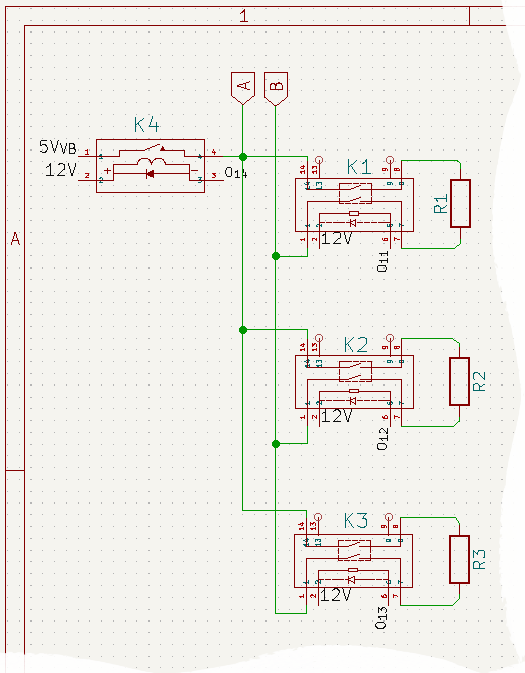
\includegraphics[width=0.6\textwidth]{figures/exemplo_reles_spst.png}
	\caption{Exemplo de utilização de relés \acrshort{spst} e \acrshort{dpst}}
	\label{fig:relespstdpst}
\end{figure}

\subsection{Registo de deslocamento}
\label{sec:hwregistodeslocamento}

\textbf{---Já foi referido com pormenor no cap3 - REFERENCIAR---}

Como já foi referido na Secção \ref{sec:registodeslocamento}, o \textit{SN74HC595} é um registo de deslocamento de 8 \textit{bits}, do tipo \acrshort{sipo}. Uma trama de (até 8) \textit{bits} é enviado pelo \gls{RaspberryPI} para o registo através do pino \acrshort{ser}. Na Figura \ref{fig:esquematico74hc595} pode ver-se o diagrama explicativo do processo de envio:

\begin{enumerate}
	\item Pinos \acrshort{oe} e \acrshort{srclr} activados;
	\item Um \textit{bit} ``0'' ou ``1'' é enviado para o pino \acrshort{ser};
	\item \textit{N} impulsos ascendentes no pino \acrshort{srclk} fazem com que o \textit{N bits} sejam enviado para o registo de deslocamento (\textit{N bits} <= 8);
	\item Um impulso ascendente no pino \acrshort{rclk} faz com que os \textit{N bits} sejam enviados para o registo de memória e, por conseguinte, para os relés (através do \textit{ULN2003A}).
\end{enumerate}

%Por cada impulso ascendente no pino \textit{SRCLK} - \textit{Shift Register Clock} - Os \textit{bits} são enviados um-a-um para o registo de deslocamento. No final, um impulso ascendente no \textit{RCLK} - \textit{Register Clock} - faz com que os \textit{bits} sejam enviados para o registo de memória e, por conseguinte, para os relés.

\begin{figure}[hbtp]
	\centering
	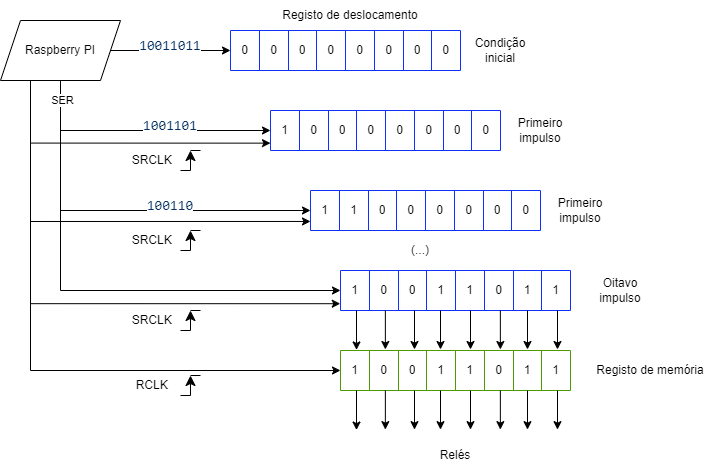
\includegraphics[width=0.7\textwidth]{figures/registo deslocamente.drawio.png}
	\caption{Envio de \textit{bits} para o registo de deslocamento}
	\label{fig:esquematico74hc595}
\end{figure}

\subsection{Driver de relés}
\label{sec:driverreles}

\textbf{---Já foi referido com pormenor no cap3 - REFERENCIAR---}
Foi referido na Secção \ref{sec:driver}, que o \gls{RaspberryPI} não tem capacidade para comandar os relés. Para isso, é necessário usar o \textit{ULN2003A} que é um \textit{driver} de relés. Na Figura \ref{fig:diagramablocos2003} está representado o diagrama simplificado para uma entrada/saída do \textit{ULN2003A} \cite{ULN2003}.

\begin{figure}[hbtp]
	\centering
	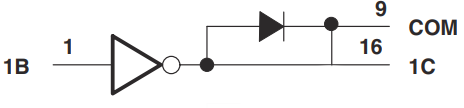
\includegraphics[width=0.6\textwidth]{figures/uln2003_diagramablocos.png}
	\caption{Diagrama de blocos simplificado do \textit{ULN2003A}}
	\label{fig:diagramablocos2003}
\end{figure}

O terminal 9 - \textit{COM} - é ligado à tensão de comando dos relés e é destinado aos díodos de ``roda livre'', conforme mencionado na Secção \ref{sec:reles}. No caso dos modelos de relés utilizados neste projecto, a tensão é de \SI{12}{\volt}.
O \textit{ULN2003A} faz parte da família dos \textit{drivers} inversores. Se o valor lógico na entrada ``1B'' = ``0'' (ou \SI{0}{\volt}), então, a saída ``1C'' = ``1'' (ou \SI{12}{\volt}).

As Figuras \ref{fig:comandorelesfull} e \ref{fig:exemplovoltimetro} servem como exemplo para ilustrar o funcionamento dos relés, em conjunto com o \textit{ULN2003A} e o \textit{SN74HC595}. Neste exemplo usou-se um relé \acrshort{spst}. No entanto, o funcionamento é idêntico para os relés \acrshort{dpst}, mudando somente os pinos.

\begin{figure}[hbtp]
	\centering
	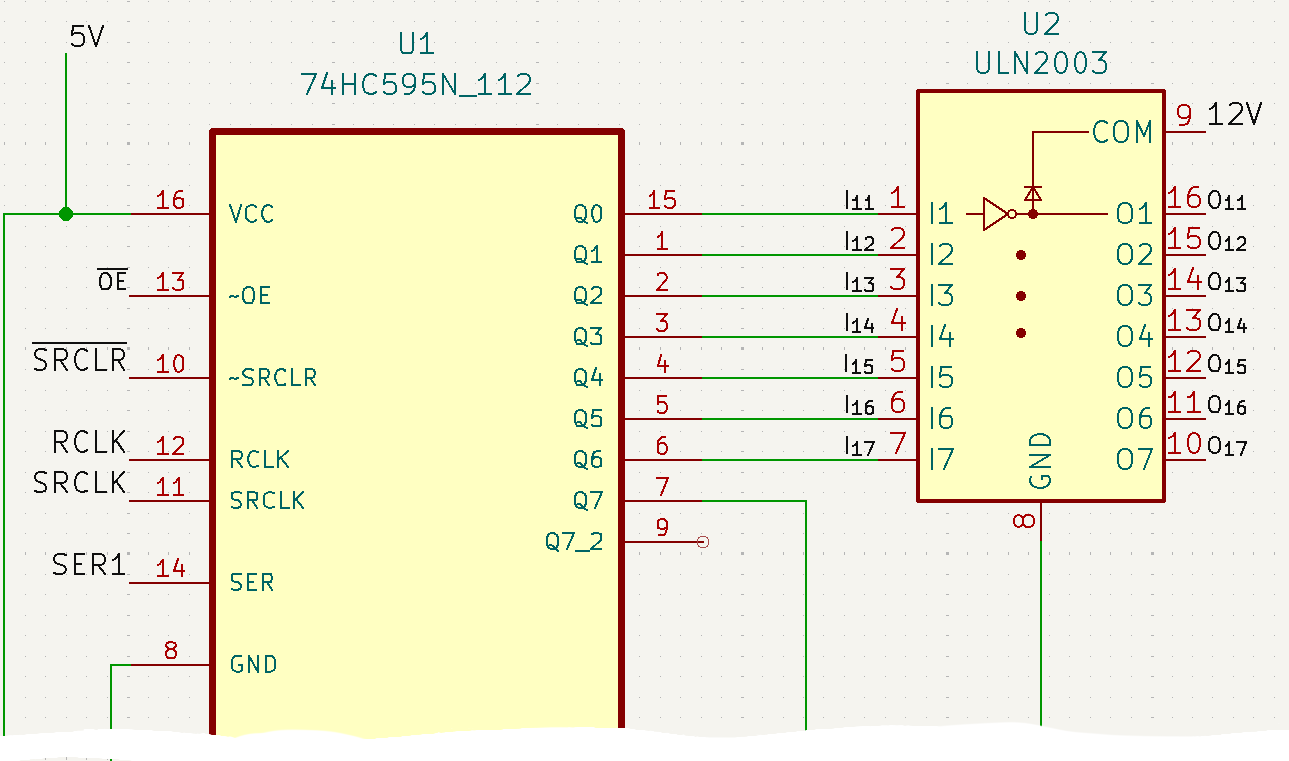
\includegraphics[width=0.7\textwidth]{figures/comandoreles_FULL.png}
	\caption{Exemplo de uso do \textit{SN74HC595} e \textit{ULN2003A} - REVER}
	\label{fig:comandorelesfull}
\end{figure}

\begin{figure}[hbtp]
	\centering
	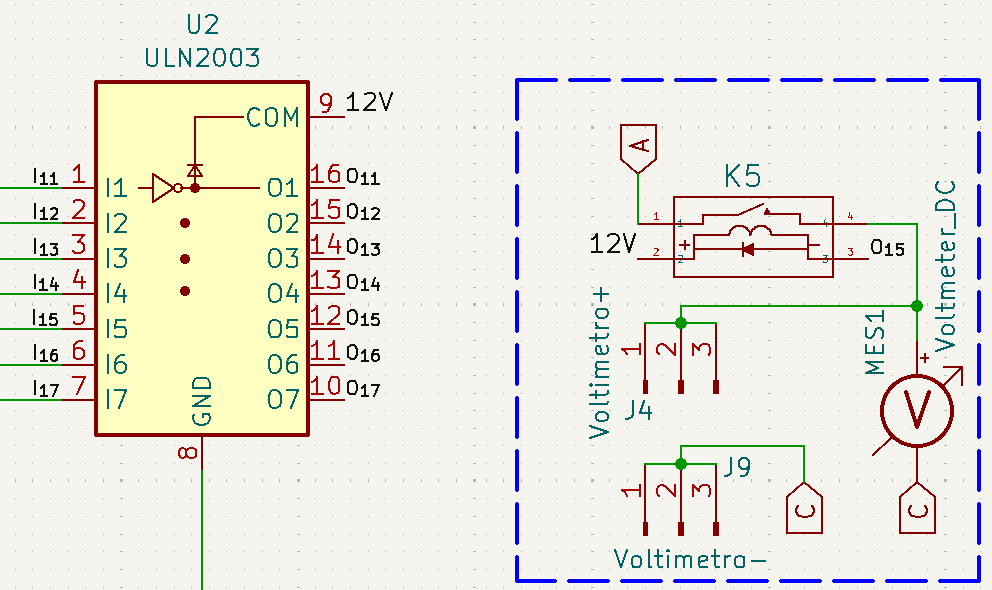
\includegraphics[width=0.7\textwidth]{figures/exemplo_voltimetro.png}
	\caption{Exemplo de comando dos relés, usando o \textit{ULN2003A}}
	\label{fig:exemplovoltimetro}
\end{figure}

As entradas $I_{1}$ a $I_{7}$ são comandadas pelo \gls{RaspberryPI}, através do registo de deslocamento - \textit{SN74HC595}, tal como apresentado na Figura \ref{fig:comandorelesfull} e as saídas $O_{1}$ a $O_{7}$ vão comandar os relés - terminais ``3'' e os terminais ``2'' dos relés são ligados aos \SI{12}{\volt}, como apresentado na Figura \ref{fig:exemplovoltimetro}.
%O funcionamento está descrito na Listagem \ref{Table:exemplouln2003}:

% \begin{table}[htb]
% 	\centering
% 	\caption{Tabela funcionamento \textit{ULN2003A} e relés}
% 	\label{Table:exemplouln2003}
% 	\begin{tabular}{ccc}
% 		\toprule
% 		\multicolumn{2}{c}{ULN2003A} & Relés                                \\
% 		\midrule
% 		Entrada                      & Saída                  & Estado      \\
% 		\midrule
% 		``0'' (\SI{0}{\volt})        & ``1'' (\SI{12}{\volt}) & Desactivado \\
% 		\midrule
% 		``1'' (\SI{12}{\volt})       & ``0'' (\SI{0}{\volt})  & Activado    \\
% 		\bottomrule
% 	\end{tabular}
% \end{table}

No caso particular do exemplo descrito em cima, se $I_{5} = I_{15}$ = \SI{0}{\volt}, então, a saída $O_{5}$ = \SI{12}{\volt} e não há diferença nos terminais ``2'' e ``3'' na bobina do relé  ``K5''. O relé está desactivado. Por outro lado, se $I_{5} = I_{15}$ = \SI{12}{\volt}, então, a saída $O_{5}$ = \SI{0}{\volt}, há diferença de potencial aos terminais da bobina e o relé está activado.

No caso em que a trama a ser transmitida for maior que 8 \textit{bits}, há a necessidade de usar mais do que um registo de deslocamento. Neste caso, o pino 9 - $Q_{H}'$ - do primeiro registo \textit{SN74HC595} é ligado ao pino \acrshort{ser} do segundo registo e assim sucessivamente.

\subsection{Fontes de alimentação}
\label{sec:fontesalimentacao}

O \acrshort{lare} utiliza várias fontes de alimentação, todas passíveis de serem controladas por \textit{software} e neste aspecto tentou-se simplificar/limitar o uso de fontes externas, além das que poderiam ser fornecidas pelo \acrshort{virtualbench}. 

Como pode ser visto na Figura \ref{fig:paineldianteiro} ou na Figura \ref{fig:promenorfontes} com mais pormenor, o \acrshort{virtualbench} possuí três fontes de alimentação (\acrshort{cc} variáveis): \SI{+6}{\volt}, \SI{+25}{\volt} e \SI{-25}{\volt}\footnote{No contexto do \acrshort{lare} a fonte de tensão negativa não é usada.}.

\begin{figure}[hbtp]
	\centering
	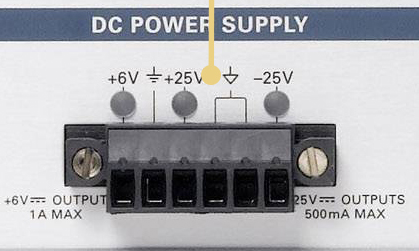
\includegraphics[width=0.7\textwidth]{figures/fontes_VB.png}
	\caption{Fontes de tensão do \acrshort{virtualbench}}
	\label{fig:promenorfontes}
\end{figure}

Assim, o \acrshort{lare} utiliza os seguintes níveis de tensão/fontes de alimentação:
\begin{itemize}
	\item \SI{1}{\volt} - \SI{5}{\volt} variáveis (\acrshort{cc}) - utilizada na experiência da Lei de Ohm;
	\item \SI{12}{\volt} (\acrshort{cc}) - utilizada na alimentação dos relés e dos \textit{drivers} de relés - ULN2003;
	\item \SI{5}{\volt} (\acrshort{cc}) - utilizada na alimentação do registo de deslocamento - 74HC595;
	\item Para o estudo dos circuitos rectificadores e filtros utilizou-se um transformador \SI{220}{\volt}/\SI{8}{\volt} \acrshort{ca}.
\end{itemize}

\subsubsection{Fonte de tensão \SI{6}{\volt} - variável}
A fonte de tensão \SI{+6}{\volt} \acrshort{cc} variável, que fornece as tensões entre \SI{1}{\volt} e \SI{5}{\volt}, para a experiência da Lei de Ohm, é obtida directamente do \acrshort{virtualbench} e ligada ao circuito tal como apresentado na Figura \ref{fig:schfonte5VB} - ``$5V_{VB}$'', terminal 1 do relé K4.

\begin{figure}[hbtp]
	\centering
	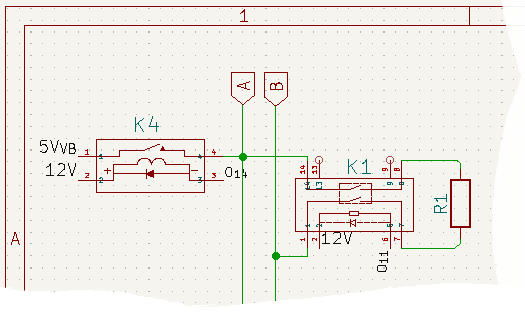
\includegraphics[width=0.7\textwidth]{figures/sch_fonte5VB.png}
	\caption{Fontes de tensão do \acrshort{virtualbench}}
	\label{fig:schfonte5VB}
\end{figure}

A configuração da fonte de \SI{6}{\volt} está exemplificada na Listagem \ref{lst:limiteI}. A variável $V_{cc}$, linha 4,  permite configurar o valor da fonte de tensão com os valores apresentados na Figura \ref{fig:pagohm}, sendo que a corrente é limitada a \SI{0.5}{\ampere}, tal como se pode ver na linha 5 da mesma Listagem.

\begin{minipage}{0.9\linewidth}
	\centering
	\begin{lstlisting}[language=Python, caption=Configuração da fonte de \SI{6}{\volt}, label=lst:limiteI]
		try:
			# Power Supply Configuration
			channel = "ps/+6V"
			voltage_level = Vcc
			current_limit = 0.5

		(...)
	\end{lstlisting}
\end{minipage}

\subsubsection{Fonte de tensão \SI{12}{\volt} - fixa}
Tal como referido em cima, de forma a simplificar o uso de fontes externas, optou-se por configurar a fonte de \SI{25}{\volt} para \SI{12}{\volt}. Esta configuração está exemplificada na Listagem \ref{lst:configfonte12} e a corrente é, também, limitada a \SI{0.5}{\ampere}, tal como se pode ver na linha 5 da mesma Listagem.

\begin{minipage}{0.9\linewidth}
	\begin{lstlisting}[language=Python, caption=Configuração da fonte de \SI{12}{\volt}, label=lst:configfonte12]
		try:
			# Power Supply Configuration
			channel = "ps/+25V"
			voltage_level = 12.0
			current_limit = 0.5

		(...)
	\end{lstlisting}
\end{minipage}

Na Figura \ref{fig:fonte12V} está representado um exemplo das ligações da fonte de \SI{12}{\volt} ao pino 9 do ULN2003 e ao pino 2 do relé ($K_{5}$)

\begin{figure}[hbtp]
	\centering
	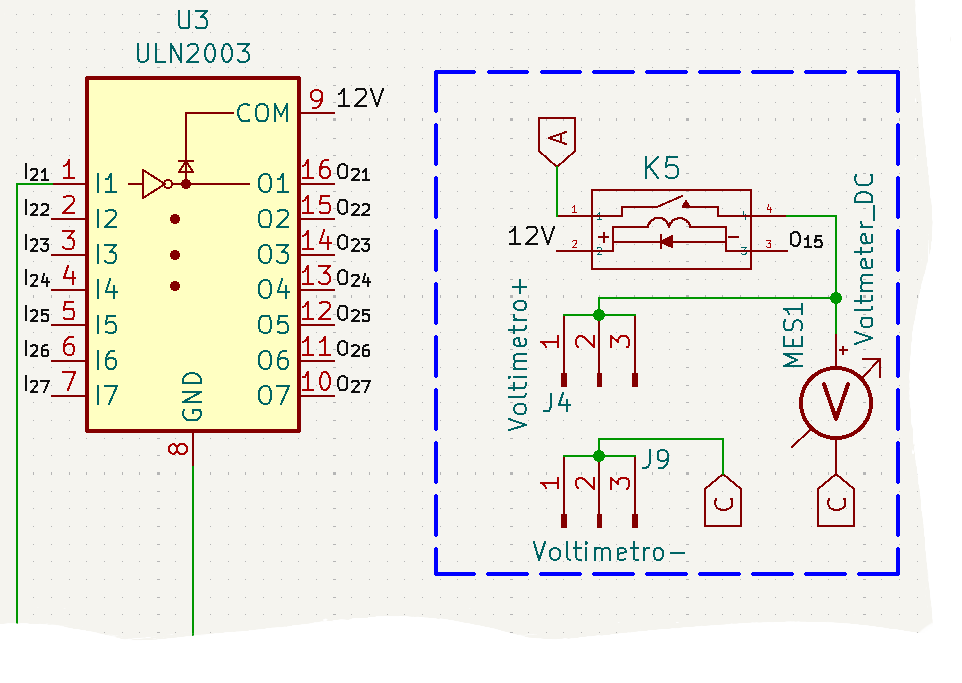
\includegraphics[width=0.8\textwidth]{figures/sch_fonte12V.png}
	\caption{Fonte de \SI{12}{\volt}}
	\label{fig:fonte12V}
\end{figure}

\subsubsection{Fonte de tensão \SI{5}{\volt} - fixa}
De forma a alimentar os circuitos com \SI{5}{\volt} fixos foi projectada uma fonte de alimentação, tal como se pode ver na Figura \ref{fig:fonte5V} \cite{LM317}.

\begin{figure}[hbtp]
	\centering
	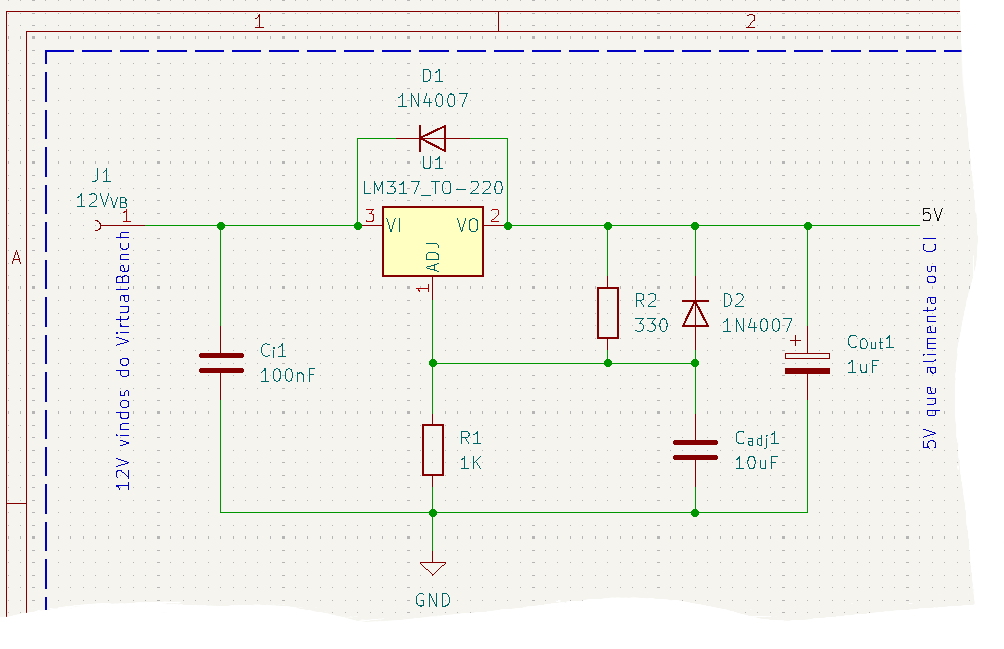
\includegraphics[width=0.8\textwidth]{figures/sch_fonte5V.png}
	\caption{Fonte de \SI{5}{\volt}}
	\label{fig:fonte5V}
\end{figure}

Esta fonte teve como base o LM317 e o esquema presente na página 11, Figura 9, do \textit{datasheet} \cite{LM317}. A utilização do LM317 em deterimento, por exemplo, do 7805 prendeu-se com a disponibilidade do regulador em contexto laboratorial. Este regulador serve perfeitamente os propósitos deste projecto, já que a tensão de saída, regulável, varia entre os \SI{1.25}{\volt} e os \SI{37}{\volt} e a corrente de saída pode ser superior a \SI{1.5}{\ampere}.

Relativamente aos díodos de protecção, $D_{1}$ e $D_{2}$, representados no esquema da Figura \ref{fig:fonte5V}, em vez de se usarem os díodos 1N4002, por uma questão de disponibilidade dos componentes, usaram-se os díodos 1N4007. Estes díodos pertencem à mesma família de diodos retificadores da série 1N400x. Ambos têm especificações elétricas e mecânicas semelhantes, nomeadamente, a capacidade de suportar correntes directas até \SI{1}{\ampere} - valor suficiente para o nosso projecto que, relembre-se, é limitado pelo \acrshort{virtualbench} a \SI{0.5}{\ampere}. No entanto, a principal diferença entre eles está na tensão inversa máxima que cada modelo é capaz de suportar \cite{1N400x}:

\begin{itemize}
	\item 1N4002: Possui uma tensão inversa máxima de 100 V;
	\item 1N4007: Suporta uma tensão inversa máxima de 1000 V.
\end{itemize}

Estes valores são, pois, mais que suficientes para os níveis de tensão usados.

Sendo assim, para uma tensão de saída de \SI{5}{\volt}, calcularam-se as resistências com base na expressão apresentada do \textit{datasheet}, representada na Equação \ref{eq:calculolm317}: 

\begin{equation} \label{eq:calculolm317}
	V_{O} = V_{REF} (1 + \frac{R_{2}}{R_{1}}) + (I_{ADJ} \times R_{2})
\end{equation}

De notar que, segundo o \textit{datasheet} do LM317 \cite{LM317}, $V_{REF} = \SI{1.25}{\volt}$ e o valor do termo $I_{ADJ} \times R_{2}$ pode ser simplificado. De facto, $I_{ADJ}$ é, tipicamente, \SI{50}{\micro\ampere}, sendo que, para o nosso projecto, o valor escolhido para $R_{2}$ foi de \SI{1}{\kilo\ohm}. Assim, segundo a Equação \ref{eq:simplificação}, tem-se que:
\begin{equation} \label{eq:simplificação}
	V_{ADJ} = I_{ADJ} \times R_{2} = \SI{0.05}{\volt}
\end{equation}

A Equação \ref{eq:calculolm317} fica então reduzida a:

\begin{equation} \label{eq:calculoR1simplificado}
	V_{O} = V_{REF} (1 + \frac{R_{2}}{R_{1}})
\end{equation}

Considerando $V_{O} = \SI{5}{\volt}$, e uma vez que a Equação \ref{eq:calculoR1simplificado} tem duas incógnitas, $R_{1}$ e $R_{2}$, atribuiu-se a $R_{2}$ o valor de \SI{1}{\kilo\ohm}, tal como foi dito anteriormente. Desta forma, obteve-se $R_{1} = \SI{333.33(3)}{\ohm}$, tal como descrito na Equação \ref{eq:calculoR1}: 

\begin{equation} \label{eq:calculoR1}
	\SI{5}{\volt} = 1.25 \times (1 + \frac{1000}{R_{1}}) \Leftrightarrow R_{1} = \SI{333.33(3)}{\ohm}
\end{equation}

O valor da resistência normalizada mais próxima é de \SI{330}{\ohm}. Importa, pois, reverter a Equação \ref{eq:calculoR1simplificado} e confirmar o valor de  $V_{O}$ obtido:

\begin{equation} \label{eq:confirmacaoVout}
	V_{O} = 1.25 \times (1 + \frac{1000}{330}) \Leftrightarrow V_{O} = \SI{5,037(87)}{\volt}
\end{equation}

Portanto, este é um valor perfeitamente aceitável para alimentar os circuitos integrados.

\subsubsection{Fontes de tensão \SI{220}{\volt}/\SI{8}{\volt} CA}
\label{sec:fontealternada}
As experiências respeitantes aos rectificadores e filtros utilizam tensão alternada sinusoidal. Tal como já foi referido anteriormente, tentou-se, sempre que possível, simplificar o uso de fontes externas. 

Na prática e em contexto de sala de aula, a experiência de rectificação de onda completa levanta um problema de massas, se se pretender usar um gerador de sinal. Quer isto dizer que não é possível medir, simultaneamente, os sinais de entrada e saída. Como se pode ver pelo esquema representado na Figura \ref{fig:gerador-massa}, o díodo está curto-circuitado (linha magenta a tracejado, entre os pontos ``2'' e ``3'') devido ao facto das massas serem comuns. 

\begin{figure}[hbtp]
	\centering
	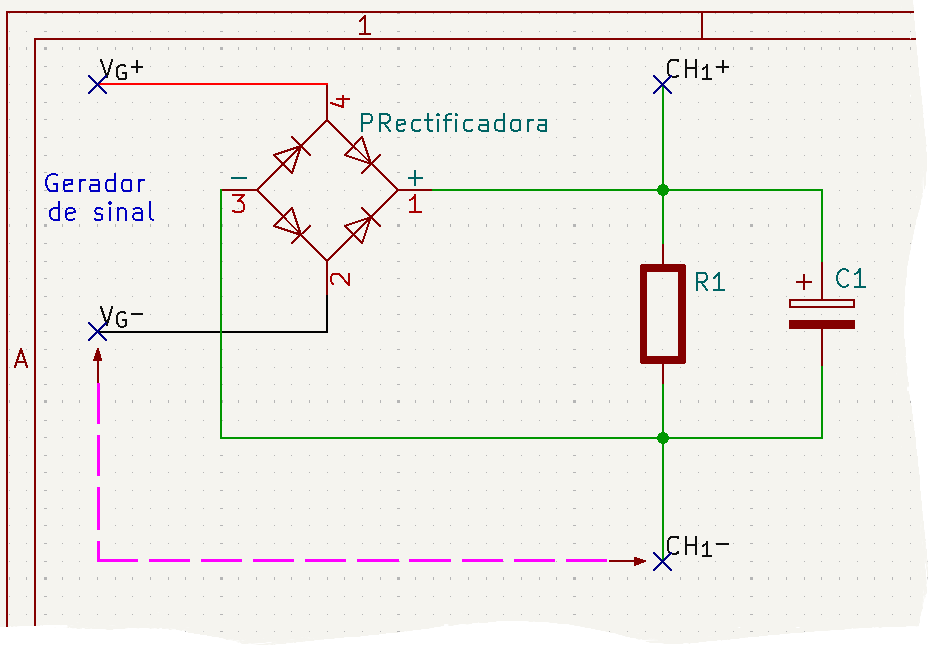
\includegraphics[width=0.8\textwidth]{figures/sch_completa_CC.png}
	\caption{Problema de massa - onda completa}
	\label{fig:gerador-massa}
\end{figure}

A forma de contornar este problema é usar um transformador e, assim, medir a onda de saída com o osciloscópio, tal como representado no esquema da Figura \ref{fig:ondacompleta-massa}. Ainda assim, não é possível medir as ondas de entrada e saída \textbf{simultaneamente}, se for esse o objectivo.

No caso do \acrshort{lare}, e com recurso ao uso de relés, é possível controlar as massas por \textit{software}. Desta forma, é possível representar as duas ondas numa imagem, tal como se pode ver na Figura \ref{fig:}. \textbf{Explicar como se fez ou deixar para a parte de software? Opinião PROF}
De referir que, desta forma, seria possível usar o gerador de sinal. No entanto, o uso do transformador justifica-se pelas seguintes razões:
\begin{itemize}
	\item Facilidade e simplicidade em controlar as massas por \textit{software} - três no caso do uso do gerador de sinal ($CH_{1-}$, $CH_{2-}$ e $VG_{-}$) ou duas no caso de se usar um transformador ($CH_{1-}$, $CH_{2-}$);
	\item Em contexto laboratorial e de sala de aula usa-se um transformador para rectificar a onda completa.
\end{itemize}

%No entanto, para o estudo da rectificação da onda completa, tal não foi possível. Enquanto que no rectificador de meia-onda (... e filtros) é possível usar o gerador de sinal do \acrshort{virtualbench} para medir as ondas de entrada e saída simultaneamente, tal não é possível na rectificação de onda completa, devido ao problema das massas e consequente curto-circuito do díodo na ponte rectificadora. 
%Este problema está representado na Figura \ref{fig:ondacompleta-massa}

\begin{figure}[hbtp]
	\centering
	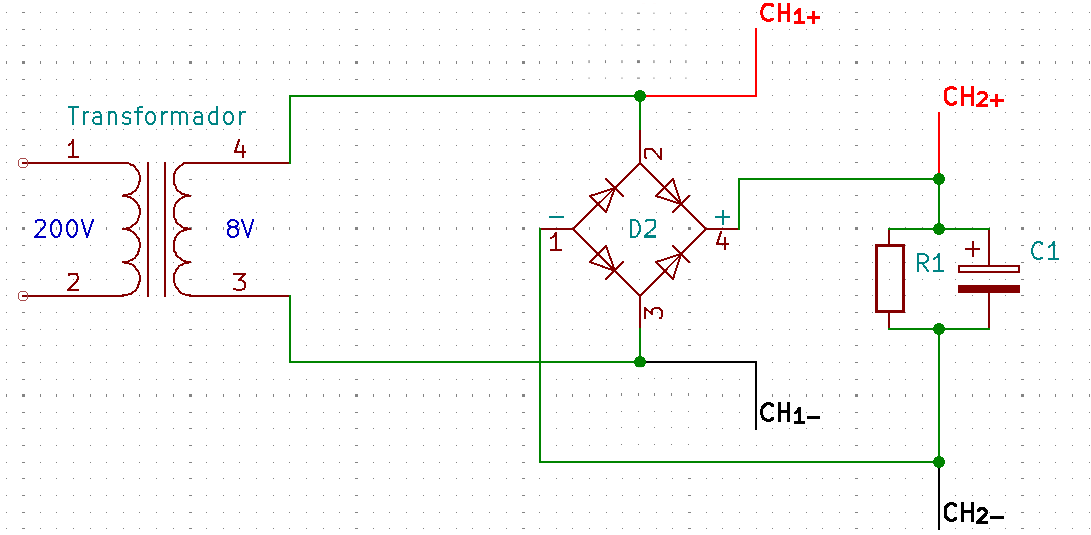
\includegraphics[width=1\textwidth]{figures/sch-ondacompleta-massa.png}
	\caption{Problema de massa - onda completa}
	\label{fig:ondacompleta-massa}
\end{figure}

O esquema completo da experiência de rectificação de onda completa pode ser consultado \textbf{no anexo, figura XPTO}.

%$CH_{1-}$ e $CH_{2-}$ são as massas do gerador de sinal e osciloscópio (dois canais), respectivamente. É fácil perceber que estando ligados ao mesmo aparelho de medida, neste caso o \acrshort{virtualbench}, as massas dos dois canais do osciloscópio são comuns e, por isso, entre os pontos 2 e 3, o díodo está curto-circuitado. 


%No que concerne à fonte de alimentação \acrshort{ca}, esta foi implementada de forma independente do \acrshort{virtualbench}. \textbf{Falar sobre a fonte de alimentação variável e a fonte de alimentação \acrshort{ca}. Colocar a foto do esquema e explicar como se faz a rectificação, cálculos inclusive. Talvez referir o facto de que depende da qualidade e valores dos transformadores e depois concluir com os valores deste caso, pode-se refferir que relativamente à fonte AC, só está disponível a fonte do gerador de sinal do VB e é mais fácil controlar através da fonte externa projectada.}

\subsection{Aparelhos de medida - voltímetro e amperímetro}
\label{sec:aparelhosmedida}

A medição de tensão e corrente são feitas utilizando o multímetro digital - \Acrfull{dmm} - PXI-4072, referenciado na Secção \ref{sec:visir}, Figura \ref{fig:PXI-4072} e cujo painel frontal está representado na Figura \ref{fig:frontDMM}.

\begin{figure}[hbtp]
	\centering
	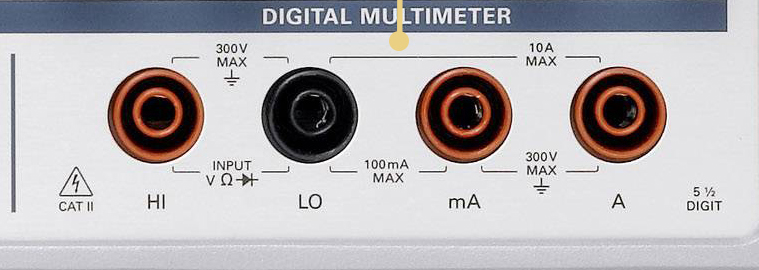
\includegraphics[width=0.7\textwidth]{figures/promenorDMM.png}
	\caption{Painel frontal Multímetro Digital}
	\label{fig:frontDMM}
\end{figure}

Os aparelhos de medida são controlados por um conjunto de relés e foram projectados de forma a serem independentes. Na Figura \ref{fig:esq_geral_ohm} está representado o esquema simplficado da Lei de Ohm que pode ilustrar o funcionamento dos aparelhos de medida. O ponto ``C'' é comum a ambos os aparelhos e é controlado pelo relé $K_{7}$. O terminal positivo do voltímetro está ligado ao ponto ``A'', controlado pelo relé $K_{5}$ mas o amperímetro necessita de mais um relé, já que o controlo da medição é diferente. Neste caso o relé $K_{8}$ funciona como um \textit{bypass} quando se pretende medir tensão e o relé $K{6}$ controla o terminal positivo do amperímetro.

De referir que, se se pretender expandir o \acrshort{lare} com mais circuitos, é possível utilizar o voltímetro e o amperímetro da forma como estão configurados. 
%Tal como pode ser visto na o voltímetro está disponível entre os pontos A e C e o amperímetro entre os pontos B e C.

A Tabela \ref{Table:exemplomedicaoohm} apresenta o estado dos relés, $K_{5}$ a $K_{8}$ consoante a grandeza que se pretende medir.

\subsection{Experiências}
\label{sec:experiencias}
Nesta secção e seguintes, considera-se, com excepção da Lei de \textit{Ohm}, que cada experiência compreende dois circuitos, isto é, a experiência da rectificação compreende o circuito de meia onda e onda completa; a experiência dos filtros compreende o circuito passa alto e passa baixo.

De forma a permitir um melhor desenvolvimento, foco, organização, detecção e correcção de erros, as experiências foram implementadas de forma independente. As primeiras ideias passavam por, além da Lei de \textit{Ohm}, implementar o estudo da rectificação de meia e onda completa. Contudo, verificou-se que seria possível incluir uma experiência adicional, dedicada ao estudo prático de filtros passa-alto e passa-baixo, já que estas duas experiências possuem componentes comuns, ampliando, assim, o alcance e a aplicabilidade do projeto.

Na Figura \ref{fig:rectificacao_filtragem_full} está representado o esquema completo e simplificado dos circuitos que compõem as duas experiências. Nele se podem ver os componentes comuns, rectângulo tracejado laranja, assim como os rectificadores de meia e onda completa, rectângulo tracejado vermelho e verde, respectivamente. Os filtros passa-alto e passa-baixo estão representados no rectângulo tracejado magenta.

\begin{figure}[hbtp]
	\centering
	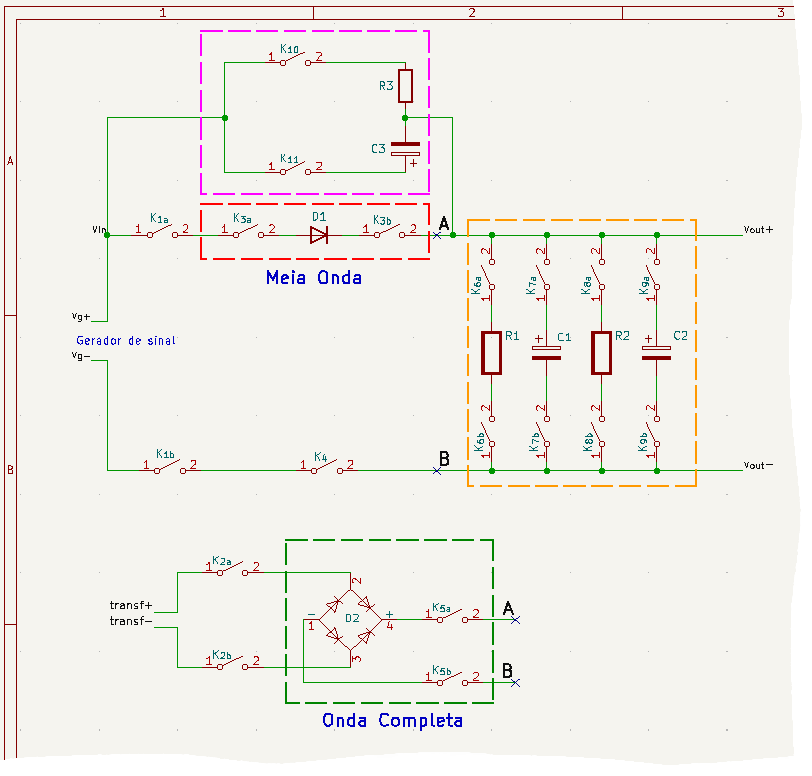
\includegraphics[width=0.7\textwidth]{figures/rec_fil_FULL.png}
	\caption{Esquema completo (simplificado) - rectificadores e filtros}
	\label{fig:rectificacao_filtragem_full}
\end{figure}

No \textit{datasheet} encontram-se os esquemas completos das experiências, assim como as placas que constituem a matriz do \acrshort{lare}: cada uma ficou dividida por uma placa, mais uma dedicada às fontes de alimentação, num total de três placas. 

\textbf{Coloca aqui, falvez, uma foto da matriz lare}

\subsubsection{Lei de Ohm}
\label{sec:lei_ohm}
\textbf{Falta o complemento com imagens do gráfico/resultado final e a imagem da placa já feita, opinião PROF}

Nesta experiência pretende-se estudar a Lei de Ohm. Na Figura \ref{fig:esq_geral_ohm} está representado o esquema simplificado do circuito - o esquema completo pode ser consultado no \textit{Datasheet}, na página ??? - \textbf{Ver como referenciar}.

\begin{figure}[hbtp]
	\centering
	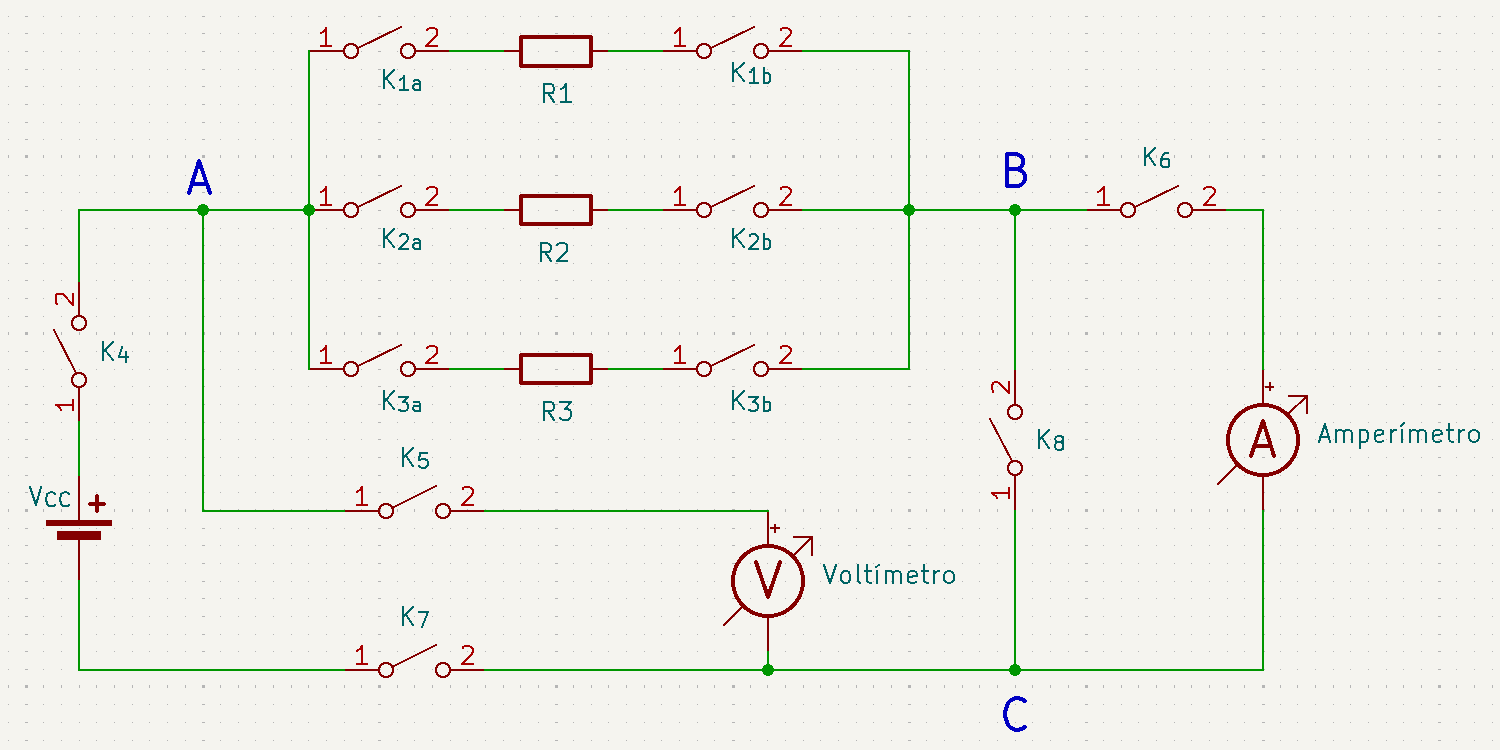
\includegraphics[width=0.7\textwidth]{figures/esquema_simplificado_OHM.png}
	\caption{Esquema simplificado da experiência Lei de Ohm}
	\label{fig:esq_geral_ohm}
\end{figure}

O funcionamento do circuito é relativamente simples. Qualquer que seja a resistência a medir, é fechado o respectivo relé - $K_{1}$ ou $K_{2}$ ou $K_{3}$; a fonte $V_{CC}$ é ligada ao circuito através do relé $K_{4}$ e $K_{7}$.

A medição da tensão e da corrente faz-se da seguinte forma:
\begin{itemize}
	\item Medição da tensão:
	      \begin{itemize}
		      \item Os relés $K_{5}$ e $K_{8}$ são fechados e $K_{6}$ é aberto (Amperímetro desactivado). Desta forma, o voltímetro fica em paralelo com a resistência a medir - entre os pontos A e B.
	      \end{itemize}
	\item Medição da corrente:
	      \begin{itemize}
		      \item Os relés $K_{5}$ e $K_{8}$ são abertos (voltíemtro desactivado) e $K_{6}$ é fechado. Desta forma, o amperímetro fica em série com a resistência a medir - entre os pontos B e C.
	      \end{itemize}
\end{itemize}

% Já foi referenciado acima
% Como se pode pode ver na Figura \ref{fig:frontDMM}, retirada da Figura \ref{fig:paineldianteiro}, o terminal negativo (preto) é comum a ambos os aparelhos de medida, que na Figura \ref{fig:esq_geral_ohm} está representado pelo ponto ``C''. O terminal positivo (vermelho) do voltímetro liga ao ponto A - depois de activo o relé $K_{5}$ e o terminal positivo (vermelho) do amperímetro liga ao ponto B - depois de activo o relé $R_{6}$.

Como exemplo, se se pretender estudar a Lei de Ohm para a resistência $R_{1}$, os relés seriam activados da forma representada na Tabela \ref{Table:exemplomedicaoohm}:

\begin{table}[htb]
	\centering
	\caption{Exemplo funcionamento de medição da Lei de Ohm} 
	
	\label{Table:exemplomedicaoohm}
	\begin{tabular}{lcccccccc}
		\toprule
		               & \multicolumn{8}{c}{Estado dos relés}                                                                       \\
		\midrule
		               & $K_{1}$                              & $K_{2}$ & $K_{3}$ & $K_{4}$ & $K_{5}$ & $K_{6}$ & $K_{7}$ & $K_{8}$ \\
		\midrule
		Medir Tensão   & 1                                    & 0       & 0       & 1       & 1       & 0       & 1       & 1       \\
		\midrule
		Medir Corrente & 1                                    & 0       & 0       & 1       & 0       & 1       & 1       & 0       \\
		\bottomrule
	\end{tabular}
\end{table}

Na Figura \ref{fig:graphohm} está representado um exemplo de um gráfico obtido com a experiência da Lei de Ohm, nos testes do \acrshort{lare}.

\begin{figure}[hbtp]
	\centering
	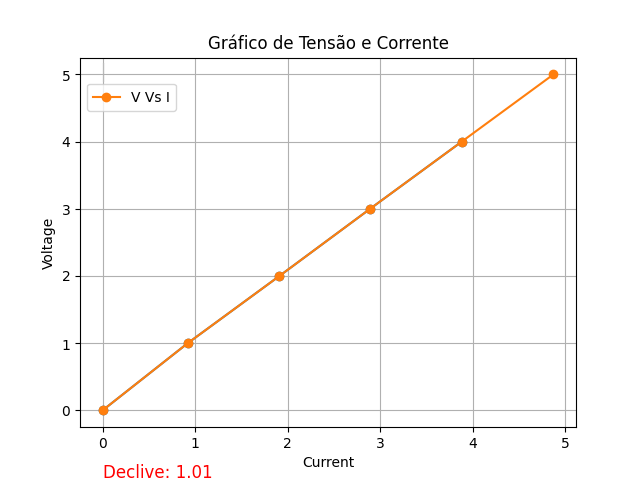
\includegraphics[width=0.6\textwidth]{figures/ohm_graph.png}
	\caption{Exemplo de gráfico Lei de \textit{Ohm}}
	\label{fig:graphohm}
\end{figure}

Da forma como está implementado, o tutor ou professor, pode optar por apresentar o conceito de duas formas distintas, em ambos os casos são efectuadas cinco medições, construido o respectivo gráfico e calculado o valor do declive da recta analiticamente. A diferença está na forma como se confrontam os resultados práticos. 

No caso em que a resistência é dada, o declive pode ser calculado e confrontado com as soluções, sendo que no caso em que é desconhecida, o declive da recta é calculado e a partir deste do resultado infere-se o valor da resistência. 

\textbf{Tal como o prof disse, refrerir que os valores, imagem, iformação e enviada para a página via xpto, blá, blá, através do ficheiro, flask, tal como referido no cap tal - referir também como é enviada a string}

\subsubsection{Rectificadores}
\label{sec:rectificadoresfiltros}

Nesta experiência pretende-se estudar e avaliar a diferença entre os dois tipos de rectificação e a influência que têm na variação da tensão de \textit{ripple}. 

Na Figura \ref{fig:blocosrectificacao} está representado o diagrama de blocos geral da rectificação de meia e onda completa, (que pode ser aplicada)/aplicada a uma fonte de tensão \acrshort{cc}, por exemplo. 

\begin{figure}[hbtp]
	\centering
	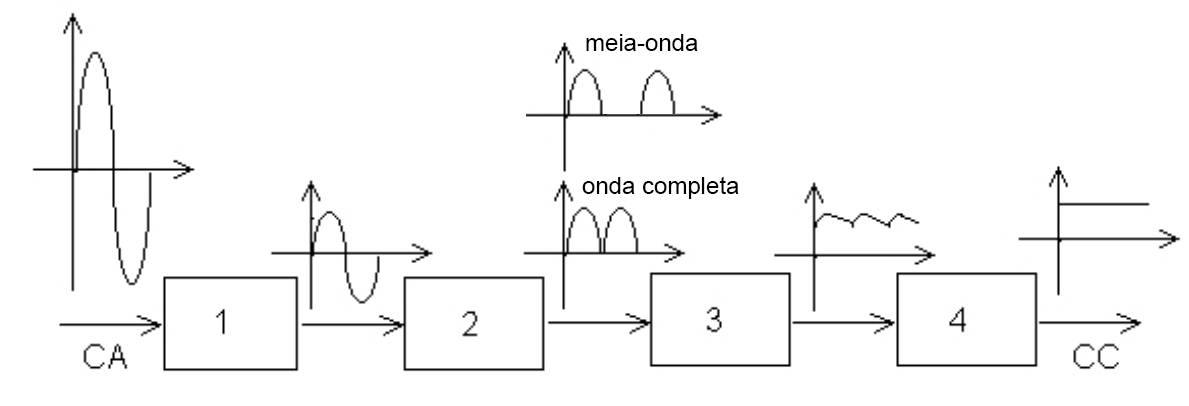
\includegraphics[width=0.8\textwidth]{figures/diagramablocosrectificacao.png}
	\caption{Diagrama de blocos geral da rectificação de meia e onda completa}
	\label{fig:blocosrectificacao}
\end{figure}

\begin{enumerate}
	\item Transformador;
	\item Rectificação;
	\item Filtragem;
	\item Estabilização.
\end{enumerate}

A tensão de \textit{ripple} é uma componente dependente do tempo que surge à saída do filtro do rectificador - Bloco 3 - sendo que terá de ser minimizada, de forma a estabilizar o valor da tensão de saída \acrshort{cc} - Bloco 4. \cite{sedrasmith} 

A Figura \ref{fig:sedraripple} representa a forma de onda à saída do Bloco 3 - Filtragem - quando se utiliza a rectificação de meia onda.
\begin{figure}[hbtp]
	\centering
	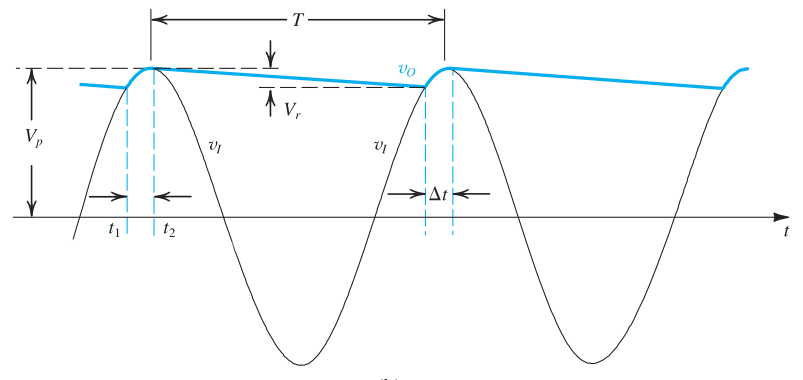
\includegraphics[width=0.7\textwidth]{figures/sedra_ripple.png}
	\caption{Forma de onda à saída do Bloco 3 - Filtragem [meia onda] \cite{sedrasmith}}
	\label{fig:sedraripple}
\end{figure}

A tensão de \textit{ripple} pode ser calculada através da Equação \ref{eq:vripple}:

\begin{equation} \label{eq:vripple}
	V_{r} = \frac{V_{P}}{fRC}
\end{equation}

Observa-se, a partir da Figura \ref{fig:sedraripple} e também da Equação \ref{eq:vripple} que, quando a constante de tempo $CR >> T$, a tensão de \textit{ripple} é pequena. Sendo que, $v_{O}$, ou seja, a tensão à saída do filtro é practicamente constante e dada pela Equação \ref{eq:tensaosaida}:

\begin{equation} \label{eq:tensaosaida}
	v_{O} = V_{P} - \dfrac{1}{2}V_{r}	
\end{equation}

No entanto, pode tornar-se este circuito mais eficiente se se usar a rectificação de onda completa e como pode ser visto na Figura \ref{fig:sedraripplecompleta}, a frequência do \textit{ripple} é o dobro da frequência da onda de entrada.

\begin{figure}[hbtp]
	\centering
	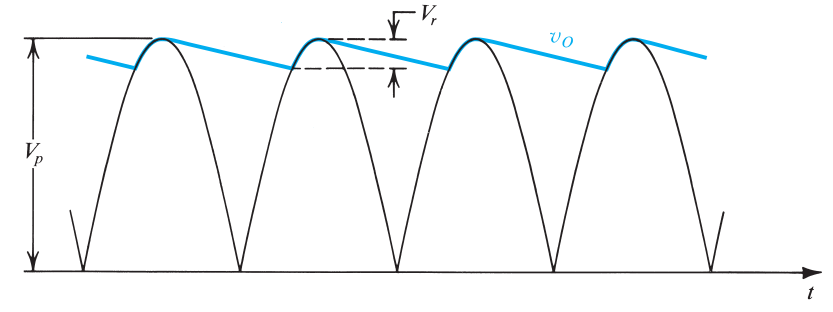
\includegraphics[width=0.7\textwidth]{figures/sedra_ripple_OC.png}
	\caption{Forma de onda à saída do Bloco 3 - Filtragem [onda completa] \cite{sedrasmith}}
	\label{fig:sedraripplecompleta}
\end{figure}

Sendo assim, o valor da tensão de \textit{ripple}, neste caso, será dado pela Equação \ref{eq:vrippleOC}:

\begin{equation} \label{eq:vrippleOC}
	V_{r} = \frac{V_{P}}{2fRC}
\end{equation}

São estas formas de onda, representadas pelas Figuras \ref{fig:sedraripple} e \ref{fig:sedraripplecompleta}, que se pretendem estudar e avaliar, assim como os valores dados pelas Equações \ref{eq:vripple} e \ref{eq:vrippleOC}.

Os esquemas simplificados que compõem os diversos blocos estão representados na Figura \ref{fig:rectificacao_filtragem_full} e tal como foi referido na Secção \ref{sec:fontealternada}, o rectificador de meia onda é alimentado pelo gerador de sinal, o que permite estudar a variação do \textit{ripple} com a frequência e o rectificador de onda completa pelo transformador monofásico - rectângulo tracejado a (...). O Bloco 3 é o único Bloco comum às duas experiências e é composto por um grupo de condensadores e resistências. (Ou "é composto pelo(s) filtro(s) definidos pelas quatro combinações dos condensadores e resistências" - ver com o prof). O Bloco 4 não está montado/projectado, visto que, como já foi dito anteriormente, o objectivo é o estudo da variação da tensão de \textit{ripple}. (A inclusão da estabilização poderá ser objecto de trabalho futuro)

Os relés foram projectados de forma a isolar totalmente os blocos dos circuitos, permitindo, assim, a sua utilização caso se pretenda expandir o \acrshort{lare} com mais experiências. No caso do gerador de sinal, este é isolado utilizando um relé duplo $K_{1}$ e o díodo é isolado através do relé duplo $K_{3}$ (rectângulo tracejado a vermelho escuro). Quanto ao relé $K_{4}$, eventualmente, seria dispensavel, já que o terminal negativo do gerador de sinal é (também) controlado por $K_{1}$. No entanto, como os filtros (rectângulo tracejado a cor-de-laranja) são comuns,  também, ao rectificador de onda completa e, caso se pretenda usar o gerador de sinal noutra experiência, optou-se, por uma questão de segurança, de isolar totalmente os componentes através do relé $K_{4}$. \textbf{Talve rever esta justificação, já que, aparentemente, o relé K4 era dispensavel.}

A implementação destas duas experiências foi feita de forma a que se possa estudar e avaliar o \textit{ripple} dos rectificadores, consoante as quatro combinações possíveis dos pares resistência/condensador. No caso da rectificação de meia onda, é ainda possível variar a frequência entre os \SI{50}{\hertz} e \SI{2000}{\hertz} mas no caso da rectificação de onda completa, a frequência é fixa ao valor da rede eléctrica - \SI{60}{\hertz}.

\textbf{Tal como o prof disse, refrerir que os valores, imagem, iformação e enviada para a página via xpto, blá, blá, através do ficheiro, flask, tal como referido no cap tal - referir também como é enviada a string}

\subsubsection{Filtros}
\label{sec:filtros}
Representados na Figura \ref{fig:filtrosesqgeral} estão os filtros simplificados, leccionados em contexto de sala de aula no ensino secundário.

\begin{figure}[hbtp]
	\centering%
		\centering
		\subfloat[\centering Filtro passa-baixo\label{fig:filtro_pb}]{{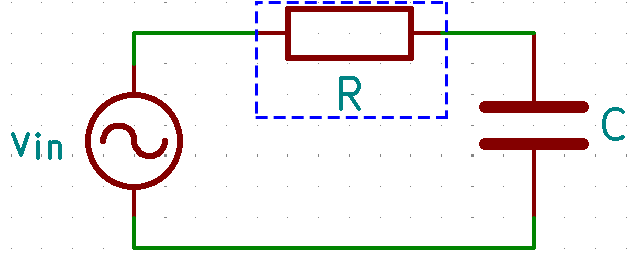
\includegraphics[width=6cm]{figures/filtro_PB_simplificado_trac.png} }}%
		\qquad
		\subfloat[\centering Filtro passa-alto\label{fig:filtro_pa}]{{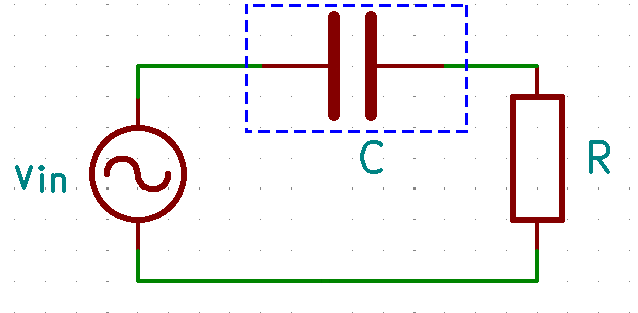
\includegraphics[width=6cm]{figures/filtro_PA_simplificado_trac.png} }}%
		\caption{Esquemas simplificados dos filtros}%
		\label{fig:filtrosesqgeral}%
	\end{figure}

A possibilidade de variar a frequência do sinal de entrada permite que estas experiências sejam utilizadas para estudar a resposta em frequência dos filtros, analisar o Diagrama de \textit{Bode}, determinar a frequência de corte dada pela Equação \ref{eq:frequenciacorte} e ainda relacionar, por exemplo, o valor da tensão de entrada com a tensão de saída. A Figura \ref{fig:diagramabode} apresenta um exemplo do Diagrama de \textit{Bode} de um filtro passa-alto, obtido nos testes do LaRE.

\begin{equation} \label{eq:frequenciacorte}
	f_{c} = \frac{1}{2\pi RC}
\end{equation}

\begin{figure}[hbtp]
	\centering
	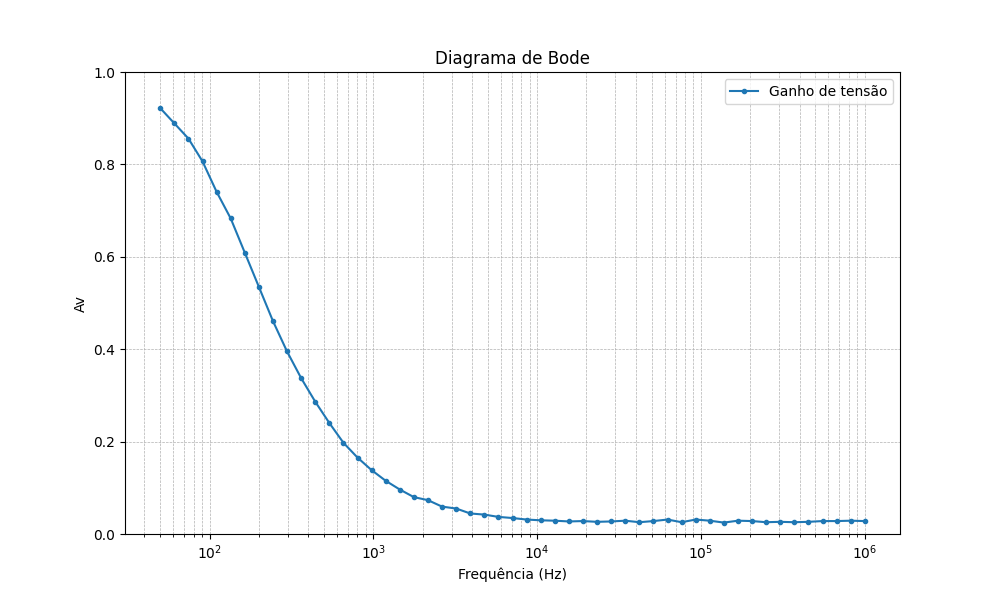
\includegraphics[width=0.6\textwidth]{figures/bode_lpf.png}
	\caption{Diagrama de \textit{Bode} - Filtro passa-alto}
	\label{fig:diagramabode}
\end{figure}

Como foi dito na Secção \ref{sec:experiencias}, a integração desta experiência foi feita após a conclusão dos rectificadores. De forma a integrar estas experiências no circuito já implementado, foi necessário realizar um \textit{bypass} ao díodo $D_{1}$ (indicado pelo retângulo tracejado vermelho na Figura \ref{fig:rectificacao_filtragem_full}). Isto permitiu a inclusão de uma resistência ou de um condensador, dependendo da versão do filtro, conforme representado na Figura~\ref{fig:filtro_pb} e Figura~\ref{fig:filtro_pa}, dentro do retângulo tracejado azul.

Com auxílio da Figura \ref{fig:rectificacao_filtragem_full} e da Tabela \ref{Table:rectificadoresfiltros}, pode ver-se o estado dos relés, respeitante a uma combinação possível para cada circuito. 

\begin{table}[htb]
	\centering
	\caption{Exemplo funcionamento do rectificador de meia onda} 
	\label{Table:rectificadoresfiltros}
	\resizebox{\columnwidth}{!}{\begin{tabular}{lccccccccccccc}
		\toprule
		               & \multicolumn{13}{c}{Estado dos relés} \\
		\midrule
		               			& $K_{1}$ & $K_{2}$ & $K_{3}$ & $K_{4}$ & $K_{5}$ & $K_{6}$ & $K_{7}$ & $K_{8}$ & $K_{9}$ & $K_{10}$ & $K_{11}$ & $K_{12}$ & $K_{13}$\\
		\midrule
		Meia Onda      			& 1		 	& 0       	& 1       & 1       & 0       & 1       & 1       & 0 	   & 0     		& 0       & 0       & 0 	   & 0 \\
		\midrule
		Onda Completa  			& 0 	 	& 1       	& 0       & 0       & 1       & 0       & 0       & 1  	   & 1    		& 0       & 0       & 1 	   & 1\\
		\midrule
		Filtro Passa-Alto      	& 1		 	& 0       	& 0       & 1       & 0       & 0       & 1       & 0 	   & 0    		& 1       & 0       & 1 	   & 1\\
		\midrule
		Filtro Passa-Baixo      & 1		 	& 0       	& 0       & 1       & 0       & 0       & 0       & 1 	   & 0    		& 0       & 1       & 1 	   & 1\\
		\bottomrule
	\end{tabular}}
\end{table}

\textbf{Tal como o prof disse, refrerir que os valores, imagem, iformação e enviada para a página via xpto, blá, blá, através do ficheiro, flask, tal como referido no cap tal - referir também como é enviada a string}

\textbf{DE UMA FORMA BREVE E RESEUMIDA, REFERIR QUANTO BITS E COMO SE FAZ A COMUNICAÇÃO COM O SER}

13 bits começar pelo esquema completo antes de dar os exemplos de funcionamento. a explicação penso que pode ficar dividida como está, mas já com o esquema e relés com os indices certos, a explicação mas os exemplos descritos em tabela só fazem sentido se for o esquema completo,

\section{Software}
\label{sec:implementacaosoftware}
Hoje em dia vive-se (n)uma Era em que toda a informação está disponível na ``ponta dos dedos'' e à distância de um \textit{click}. A pesquisa, desenvolvimento e teste dos assuntos mais técnicos revelou-se longa e muitas vezes extenuante. Os recursos são (quase) incomensuráveis e o grande desafio foi tentar perceber a dicotomia certo/errado. Recorreu-se à Inteligência Artificial, documentação técnica \textit{online}, fóruns de discussão, ajuda pessoal, tutoriais \textit{online} e vídeos no YouTube.

Este projeto de código fonte aberto está dividido em dois repositórios, disponíveis para consulta e modificação sob a licença GPL-3.0 (GNU General Public License, versão 3) no GitHub: \href{https://github.com/eddygrinder/LaRE}{LaRE} e \href{https://github.com/eddygrinder/LaRE_PICode}{PiCode}. Assim, os ficheiros são referenciados relativamente ao respectivo repositório. Ao longo deste capítulo, sempre que se justificar e para fins de clareza, será apresentado o código necessário - em pequenos trechos - de forma a melhor ilustrar os conceitos discutidos.

\subsection{Servidor Flask}
\label{sec:flask}
\textbf{Não sei se ainda vai ficar desta forma - no cap anterior já foi falada sobre a escolha do flask, por isso não faz sentido abordar novamente.}

Na Secção \ref{sec:back-end} foram já referidas as razões que levaram à escolha do \textit{Flask} como servidor \textit{web}. 

A base para a implementação do \textit{Flask} e \underline{\textbf{toda a informação descrita no}} \underline{\textbf{Capítulo \ref{sec:implementacaosoftware}}} teve como base e referência a documentação técnica disponível no \textit{site} do \href{https://flask.palletsprojects.com/en/3.0.x/}{\textit{Flask}} e complementada com alguns tutoriais do \textit{Youtube}, como por exemplo: \href{https://www.youtube.com/watch?v=dam0GPOAvVI}{\textit{link}} ou \href{https://www.youtube.com/watch?v=bB6Yyh7nUl4}{\textit{link}} .

\subsubsection{Estrutura base}
O fluxograma apresentado na Figura \ref{fig:funcflask} apresenta o funcionamento geral do servidor \textit{Flask}.

\begin{figure}[hbtp]
	\centering
	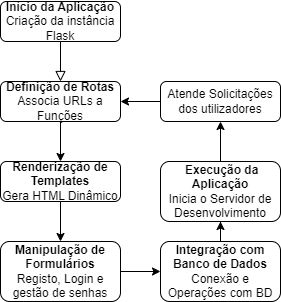
\includegraphics[width=0.7\textwidth]{figures/fluxograma_flask.drawio.png}
	\caption{Funcionamento geral \textit{Flask}}
	\label{fig:funcflask}
\end{figure}

A estrutura de directórios do \textit{Flask} tem uma base pré-definida que não é necessariamente rígida e pode ser adaptada consoante os requisitos do projecto \cite{Flask}. No caso do \acrshort{lare} a estrutura ficou organizada da forma como se mostra na Figura \ref{fig:estruturapastas}

\begin{figure}[hbtp]
	\centering
	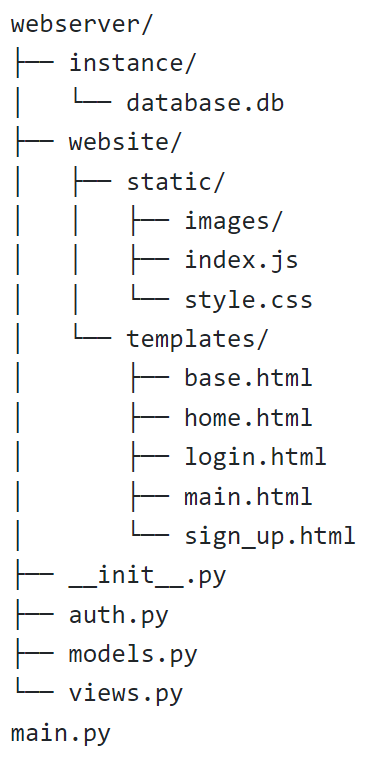
\includegraphics[width=0.3\textwidth]{figures/tree_flask.png}
	\caption{Estrutura de directórios - \textit{Flask} \textbf{ main.html está a mais}}
	\label{fig:estruturapastas}
\end{figure}

A raiz do projecto é o directório ``\textit{webserver}'' e nele estão contidos o ficheiro principal, assim como outros directórios e ficheiros de configuração essenciais:
\begin{itemize}
	\item \textit{main.py}: O ficheiro principal do aplicativo que inicializa e configura o \textit{Flask};
	\item \textit{requirements.txt}: Uma lista de dependências do projeto que podem ser instaladas usando \gls{pip};
	\item \textit{static/}: Este diretório contém os ficheiros estáticos como \acrshort{css}, \textit{JavaScript} e as imagens usadas em toda a aplicação;
	\item \textit{templates/}: Contém os modelos \acrshort{html} usado para renderizar as visualizações;
	\item \textit{instance/}: Diretório para armazenar ficheiros de configuração ou ficheiros que mudam em tempo de execução, específicos da cada instância, por exemplo, ficheiros da base de dados.
\end{itemize}

Dentro da raiz, criou-se o directório \textit{website} onde se incluiu os ficheiros respeitantes ao funcionamento do \textit{site}. Nele constam os já descritos \textit{templates}, \textit{static} e ainda os seguintes ficheiros:

\begin{itemize}
	\item \textit{\_\_init\_\_.py}: Inicializa o \textit{Flask} e define as configurações. Este ficheiro dentro da directoria \textit{website} faz com que esta seja tratada como um pacote \textit{Python}. Isto quer dizer que a directoria pode ser importada e tudo o que estiver dentro é executado automaticamente;
	\item \textit{views.py}: Contém as funções de visualização para o tratamento de pedidos \acrfull{http};
	\item \textit{models.py}: Define os modelos de dados para a aplicação;
	\item \textit{auth.py}: Este ficheiro é responsável por lidar com a autenticação e autorização de utilizadores, pode incluir funções e rotas que permitem aos utilizadores registarem-se, fazer \textit{login} e fazer \textit{logout}.
\end{itemize}

\subsubsection{Rotas}
As aplicações \textit{Web} modernas utilizam \acrshort{url}s amigáveis para ajudar os utilizadores a memorizar e utilizar o nome para voltar a visitar diretamente uma página.

No \textit{Flask} utiliza-se o decorador \textit{\textbf{route()}} para associar uma função a um \acrshort{url}, tal como pode ser visto na Listagem \ref{lst:decoradorroute}.

\begin{minipage}{0.9\linewidth}
	\begin{lstlisting}[language=Python, caption=Decorador \textit{route()} - \textit{views.py}, label=lst:decoradorroute]
@views.route("/ohm", methods=['GET', 'POST'])
@login_required
def pagina_seguinte():
    return render_template("ohm.html", user=current_user)
\end{lstlisting}
\end{minipage}

O decorador \textit{\textbf{route}} define uma rota para a \acrshort{url} \textit{ohm}. Esta rota aceita pedidos \acrshort{http} de métodos \textit{GET} e \textit{POST}.

O decorador \textit{\textbf{login}} garante que o utilizador tem de estar autenticado para aceder a esta rota. Se o utilizador não estiver autenticado, será redirecionado para a página de \textit{login}.

A função pagina\_seguinte() é executada assim que a respectiva rota for acedida.

A última linha renderiza o \textit{template} \textit{\textbf{home.html}} e passa o objecto \textit{current\_user} para o \textit{template}.

Para construir um \acrshort{url} para uma função específica, usa-se a função \textit{\textbf{url\_for()}}. Esta função aceita o nome da função como seu primeiro argumento e qualquer número de argumentos de palavras-chave, cada um correspondendo a uma parte variável da regra de \acrshort{url}, tal como pode ser visto na Listagem \ref{lst:urlfor}

\begin{minipage}{0.9\linewidth}
	\begin{lstlisting}[language=Python, caption=Contrução de \textit{url}s - \textit{auth.py}, label=lst:urlfor]
(...)
if user:
    if check_password_hash(user.password, password):
        flash('Logged in successfully!', category='success')
        login_user(user, remember=True)
        return redirect(url_for('views.home'))
(...)
\end{lstlisting}
\end{minipage}

Isto quer dizer que o \textit{Flask} gera a \acrshort{url} correspondente à função \textit{\textbf{home()}} definida no ficheiro \textit{\textbf{views.py}} dentro da \textit{Blueprint} \textit{views}. Quando usada dentro de \textit{\textbf{redirect}}, redireciona o utilizador para essa \acrshort{url}.

\subsubsection{Blueprints}
O \textit{Flask} usa um conceito de \textit{blueprints} para criar componentes de aplicações e suportar padrões comuns dentro de uma aplicação ou entre aplicações. As \textit{blueprints} podem simplificar muito o funcionamento de grandes aplicações e fornecer um meio central para que as extensões do \textit{Flask} registem operações em aplicações. As \textit{blueprints} permitem organizar a aplicação em partes menores e de mais fácil gestão. O conceito básico das \textit{blueprints} é que registam as operações a executar quando são integrados numa aplicação. O \textit{Flask} associa funções de vista (\textit{views}) a \textit{blueprints} quando processa pedidos e gera \acrshort{url} entre diferentes pontos de acesso.

Na Listagem~\ref{lst:blueprintviews} e Listagem~\ref{lst:blueprintauth} podem ver-se as duas \textit{blueprints} definidas no caso da implementação do \acrshort{lare}.
\begin{center}
	\begin{minipage}{0.7\linewidth}
		\begin{lstlisting}[language=Python, caption=\textit{Blueprint views} - \textit{views.py}, label=lst:blueprintviews]
views = Blueprint('views', __name__)
\end{lstlisting}
	\end{minipage}
\end{center}

\begin{center}
	\begin{minipage}{0.7\linewidth}
		\begin{lstlisting}[language=Python, caption=\textit{Blueprint auth} - \textit{auth.py}, label=lst:blueprintauth]
auth = Blueprint('auth', __name__)
\end{lstlisting}
	\end{minipage}
\end{center}

Ambas as \textit{blueprints} são registadas no ficheiro \textit{\_\_init\_\_.py}, como se pode verificar na Listagem \ref{lst:initreg}

\begin{center}
	\begin{minipage}{0.7\linewidth}
		\begin{lstlisting}[language=Python, caption=Registo das \textit{blueprints} - \textit{\_\_init\_\_.py}, label=lst:initreg]
app.register_blueprint(views, url_prefix='/')
app.register_blueprint(auth, url_prefix='/')
\end{lstlisting}
	\end{minipage}
\end{center}

Isto quer dizer que ao registar a \textit{blueprint} com o prefixo ``/'', os \acrshort{url}s serão acessíveis através da raiz da aplicação.

\subsubsection{Pedidos}
A capacidade de uma aplicação \textit{web} em responder a solicitações de dados do cliente é um requisito essencial. No \textit{Flask} esta informação é fornecida pelo objeto global \textit{\textbf{request}}. Este objeto contém todos os detalhes da solicitação, como os métodos \acrshort{http} usados (\textit{GET}, \textit{POST}, etc.), os \textit{headers} os \textit{cookies} ou o corpo da requisição.

O método de requisição pode ser determinado através do atributo \textit{\textbf{method}}. Para aceder aos dados de um formulário (transmitidos numa requisição \textit{POST} ou \textit{PUT}), utiliza-se o atributo \textit{\textbf{form}}, tal como descrito no ficheiro auth.py.

Quando se adiciona um ponto de interrogação (?) seguido de pares chave-valor (key=value) no final de um \acrshort{url}, está a enviar-se dados adicionais ao servidor, esses dados são chamados de \textbf{parâmetros do \acrshort{url}}, como se pode ver na Listagem \ref{lst:paramurl}.

\begin{minipage}{0.9\linewidth}
	\begin{lstlisting}[language=Html, caption=Exemplo argumentos passados ao servidor - ohm.html, label=lst:paramurl]
const url = `/config_VirtualBench?parameter=${parameter}&Vcc=${Vcc}&R=${Resistance}`;
\end{lstlisting}
\end{minipage}

No entanto, a criação e renderização das páginas \acrshort{html} é feita automaticamente através dos modelos \textit{Jinja2}\footnote{A documentação pode ser consultada em \href{https://jinja.palletsprojects.com/en/3.1.x/templates/}{\textit{Jinja}}}. Os modelos podem ser usados para gerar qualquer tipo de ficheiro de texto, sendo que para aplicações \textit{web} serão, principalmente, páginas \acrshort{html}.

No ficheiro base.html, pode ver-se a combinação entre código \acrshort{html} e sintaxe \textit{Jinja2}.

No código \acrshort{html}, encontram-se secções entre chavetas {} com palavras-chave especiais como por exemplo {\% block \%} e {\% endblock \%}. Estes são blocos de modelo \textit{Jinja2} que definem áreas de conteúdo dinâmico que podem ser preenchidas com lógica ou dados em \textit{Python}. Para renderizar um modelo, o método utilizado foi \textit{\textbf{render\_template()}} \cite{Flask}. O \textit{Flask} procurará por modelos na pasta \textit{templates}, como pode ser visto na Figura \ref{fig:estruturapastas}.

Na página oficial do \textit{Flask} é recomendado que se aceda aos parâmetros do \acrshort{url} com \textit{\textbf{get}} ou capturando o \textit{\textbf{KeyError}}, uma vez que os utilizadores podem alterar o \acrshort{url} e, nesse caso, apresentar uma página \textit{400 bad request} não é de fácil interpretação. \textbf{ATENÇÃO: Verificar se será preciso desenvolver mais este parágrafo - OPINIÃO PROF}

\subsubsection{Base de dados}
A aplicação desenvolvida usa uma base de dados e autenticação de utilizador, a ligação com a base de dados é aberta no início do pedido e é obtida a informação do utilizador. No final do pedido, a ligação com a base de dados é fechada.

No contexto da documentação do \textit{Flask} e implementação de uma base de dados, são apresentados duas alternativas: \textit{SQLite 3} e \textit{SQLAlchemy}. Tal como referenciado/aconselhado na documentação, usou-se a extensão \textit{Flask-SQLAlchemy}, descrita no ficheiro \textit{\textunderscore\textunderscore init.py\textunderscore\textunderscore}.

\subsubsection{Autenticação}
A segurança da aplicação é assegurada através das funcionalidades de \textit{login} e \textit{logout}, implementadas no ficheiro \textit{auth.py}. Para tal, foi instalada a extensão \textit{flask-login}.

Esta extensão facilita a gestão de sessões de utilizadores, permitindo manter o estado autenticado entre diferentes requisições, fornecendo métodos como \textbf{\textit{login\textunderscore user()}}, \textbf{\textit{logout\textunderscore user()}} e \textbf{\textit{current\textunderscore user}}, que simplificam a verificação do estado de autenticação. O processo de registo envolve a recolha de credenciais, como nome de utilizador e senha, garantindo o armazenamento seguro da senha através de \textbf{\textit{hashing}} com \textbf{\textit{generate\textunderscore password\textunderscore hash}}. No \textit{login}, a aplicação verifica as credenciais fornecidas, compara a senha inserida com a armazenada usando \textbf{\textit{check\textunderscore password\textunderscore hash}} e, se for válida, inicia a sessão do utilizador. Além disso, certas rotas são protegidas para garantir que apenas utilizadores autenticados as possam aceder, utilizando o decorador \textbf{\textit{@login\textunderscore required}}, que redireciona utilizadores não autenticados para a página de \textit{login}. A gestão de sessões é feita através de \textit{cookies} seguros, permitindo ainda a funcionalidade de lembrar a sessão entre reinícios do navegador, caso seja activado o parâmetro \textbf{\textit{remember=True}} no \textbf{\textit{login\textunderscore user}}. 

Devido à complexidade da implementação de uma verificação por \textit{email}, a aplicação restringe-se à autenticação baseada apenas no nome de utilizador e senha. A inclusão desse mecanismo exigiria um serviço de envio de \textit{emails} e a gestão de \textit{tokens} de confirmação.

\textbf{A REVER: Valerá a pena uma página de admin, de forma a que o professor, por exemplo faça os registo e forneça os dados de acesso aos alunos?}

\subsection{Páginas \textit{Web}}
\label{sec:paginas}
\textbf{DÚVIDA - Não sei se esta parte estará bem enquadrada}

Como mencionado na Secção \ref{sec:frontend}, procurou-se manter a experiência de utilização e navegação o mais simples, prática e intuitiva possível.

Além das páginas que compõem a base do \textit{site}, representadas na Figura \ref{fig:estruturapastas}, há ainda a juntar as que permitem ao utilizador interagir com as experiências do \acrshort{lare}. Especificamente, foram implementadas cinco páginas, correspondentes aos cinco circuitos definidos na Secção \ref{sec:solucaoproposta}.

O menu de escolha foi retirado do \textit{site} \href{https://www.w3schools.com/howto/howto_js_vertical_tabs.asp}{\textit{w3schools}} e modificado de acordo com as necessidades do projecto, tal como pode ser visto, por exemplo, na Figura \ref{fig:pagmenu}.

\begin{figure}[hbtp]
	\centering
	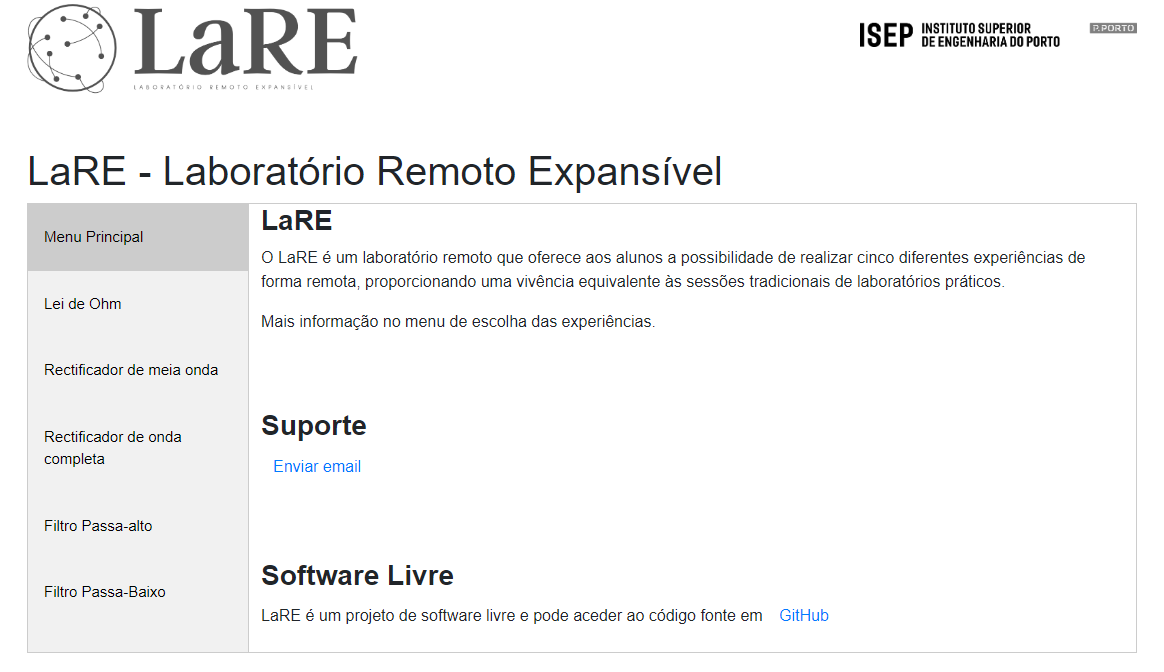
\includegraphics[width=0.7\textwidth]{figures/menupage.png}
	\caption{Página inicial}
	\label{fig:pagmenu}
\end{figure}

A navegação ficou dividida da seguinte forma:
\begin{itemize}
	\item Autenticação;
	\begin{itemize}
		\item Menu Principal;
		\begin{itemize}
			\item Página introdutória da experiência;
			\begin{itemize}
				\item Página de controle e realização da experiência.
			\end{itemize}
		\end{itemize}
	\end{itemize}
\end{itemize}

A título de exemplo, a página sobre a Lei de \textit{Ohm}, que é apresentada ao utilizador, está representada na Figura \ref{fig:ohm_intro}.

O passo seguinte é a página de controlo e realização da experiência, como se pode ver na Figura \ref{fig:ohm_ctrl}. Os selectores dos parâmetros ``$V_{CC}$'' e ``R'' estão inicialmente desabilitados. Seleccionando ``OK'' as opções ficam disponíveis. Seleccionando ``STOP/RESET'' a experiência é interrompida e os selectores ficam desabilitados.

\begin{figure}[hbtp]
	\centering%
		\centering
		\subfloat[\centering Introdução\label{fig:ohm_intro}]{{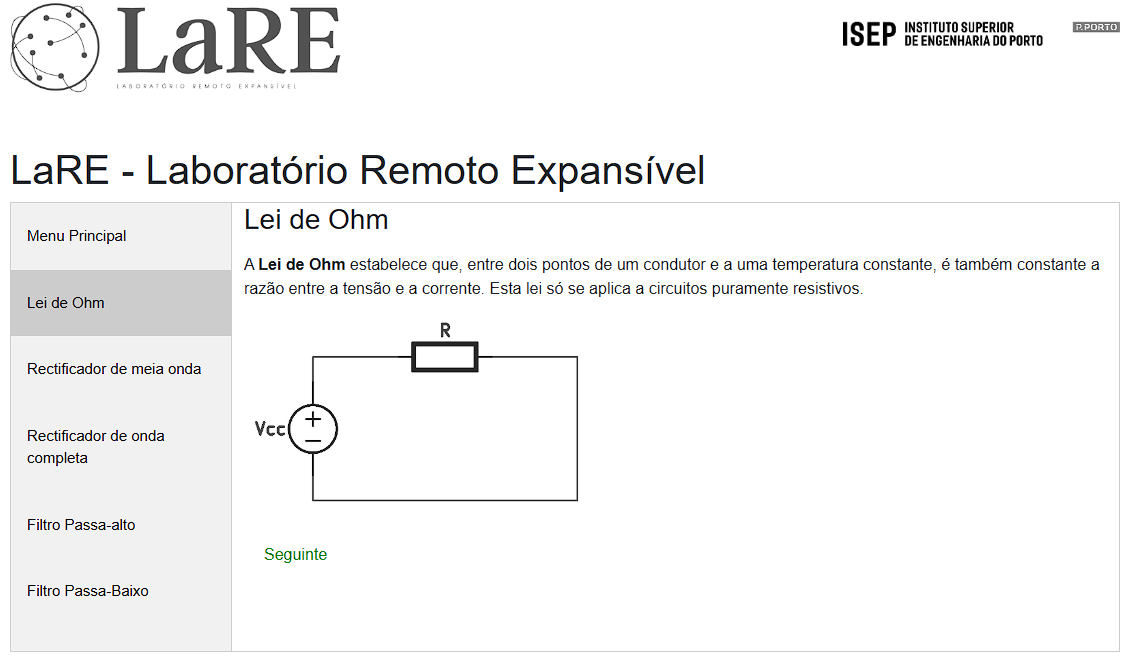
\includegraphics[width=6cm]{figures/ohm_page.png} }}%
		\qquad
		\subfloat[\centering Controlo\label{fig:ohm_ctrl}]{{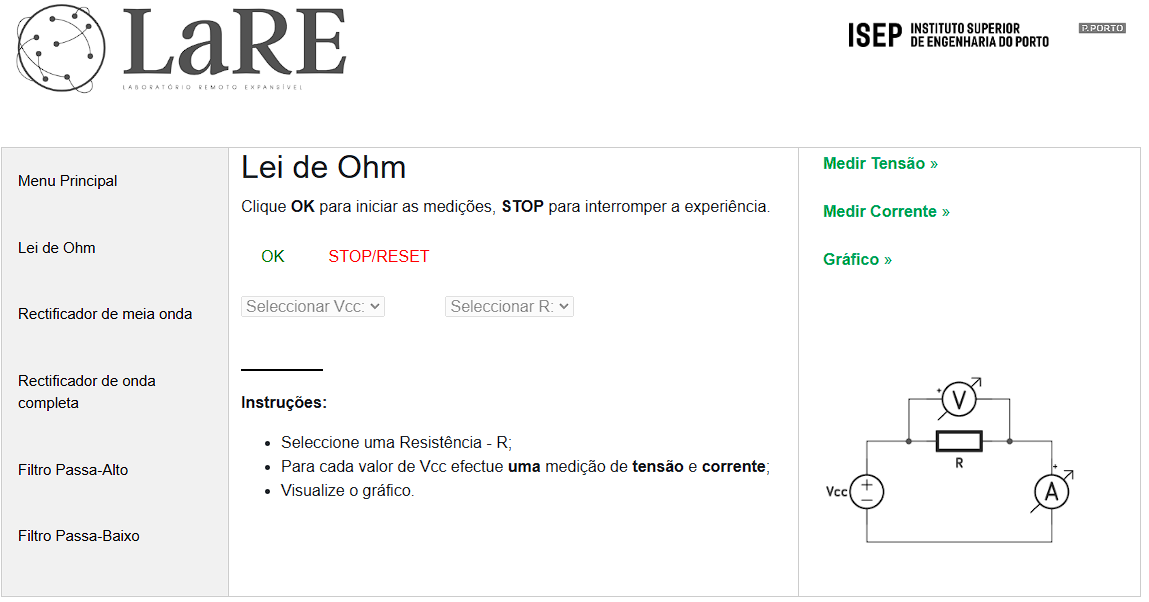
\includegraphics[width=6cm]{figures/ohm_page_controlo.png} }}%
		\caption{Experiência Lei de \textit{Ohm}}%
		\label{fig:pagohm}%
	\end{figure}

As outras experiências seguem a mesma estrutura de menus e o mesmo padrão de organização e navegação.

\subsection{Arquitectura de Comunicação}
\label{sec:comunicacao}
Nesta secção, o foco será analisar a comunicação (e troca de parâmetros) entre os diversos tipos de ficheiros. Na Figura \ref{fig:diagramasimplificado} é apresentado o diagrama simplificado que ilustra o funcionamento geral deste tipo de comunicação. 

\begin{figure}[hbtp]
	\centering
	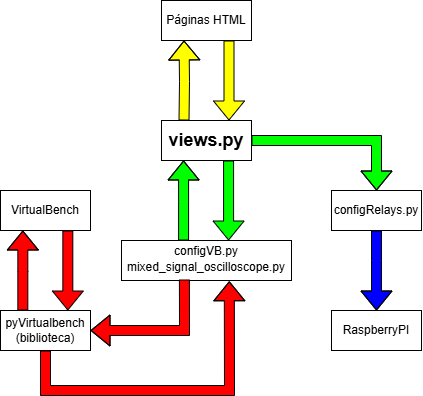
\includegraphics[width=0.7\textwidth]{figures/Diagrama_simplificado.drawio.png}
	\caption{Diagrama de comunicação simplificado [REVER]}
	\label{fig:diagramasimplificado}
\end{figure}

A arquitectura do sistema é composta por multiplos ficheiros que comunicam entre si, englobando a troca de parâmetros. O critério utilizado foi o de manter o ficheiro \textit{views.py} o mais leve e simples possível, mantendo-se o comando e controlo dos dispostivos em ficheiros separados.

Como mencionado na Secção \ref{sec:flask}, a estrutura de directórios do \textit{Flask} possui uma base pré-definida, mas suficientemente flexível para ser adaptada conforme os requisitos específicos do projeto, como ilustrado na Figura \ref{fig:estruturapastas}. De uma forma geral, foram criados ficheiros específicos para cada experiência, adoptando o critério de evitar uma excessiva modularização do código. Embora esta prática ofereça vantagens, também apresenta as suas desvantagens - devido à fragmentação excessiva - já que pode tornar a compreensão e manutenção do código mais complexa.

Os seguintes ficheiros foram criados e associados às respectivas experiências:

\textbf{Específicos}
\begin{itemize}
	\item Lei de \textit{Ohm} - \textit{config.py};
	\item Rectificadores/Filtros - \textit{mixed\_signal\_oscilloscope.py};
	\item \textins{ohm, meiaonda, ondacompleta, passaalto, passabaixo}.html.
\end{itemize}

\textbf{Comuns}
\begin{itemize}
	\item \textit{views.py} - parte central da aplicação, pois nele estão definidas todas as rotas \textit{Flask}. Quer isto dizer que, cada roda representa uma funcionalidade ou página \textit{web} específica e qualquer troca de dados ou argumentos entre ficheiros e/ou \textit{scripts}, passa obrigatoriamente por este ficheiro. Sendo assim, tentou-se, sempre que possível, reduzir o código ao estritamente necessário;
	\item \textit{configRelays.py} - ficheiro responsável pelo envio da trama de \textbf{bits} para o \textit{RaspberryPI}.
	\item \textins{login, base, sign\_up}.html - páginas de autenticação e registo de utilizadores.
\end{itemize}

Sendo assim, a comunicação entre as páginas \acrshort{html} e o ficheiro \textit{python}\footnote{Pode-se, neste caso, reduzir a comunicação ao caso mais geral de troca de informação entre ficheiros \acrshort{html} e \textit{python}, já que, no fundo, o ficheiro \textit{views.py} está escrito em \textit{python}.} é feita nos dois sentidos - setas amarelas - já que os utilizadores enviam os parâmetros específicos de cada experiência e os resultados são apresentados nas páginas. A Listagem \ref{lst:htmlpy} ilustra a forma como os parâmetros são enviados da página \acrshort{html} para o ficheiro \textit{python} - Linha \ref{line:parametros} - e como os resultados são recebidos - Linha \ref{line:resultado}.

\textbf{Aqui poderia ficar o parágrafo da explicação do ?}

\begin{minipage}{0.9\linewidth}
	\begin{lstlisting}[language=html, escapechar=|, caption=Comunicação \acrshort{html} - \textit{views.py}, label=lst:htmlpy]
	const url = `/config_VirtualBench?variavel_1=${parametro_1}&variavel_2=${parametro_2}&variavel_3=${parametro_3}`; |\label{line:parametros}|
	(...)
	document.getElementById("variavel").innerHTML = data.resultado + " V"; |\label{line:resultado}|
	\end{lstlisting}
\end{minipage}

O envio de parâmetros para as páginas é feito em \acrfull{json}, usando a instrução definida na Listagem \ref{lst:returnjson}.

\begin{minipage}{0.9\linewidth}
	\begin{lstlisting}[language=python, escapechar=|, caption=Comunicação \textit{views.py} - \acrshort{html}, label=lst:returnjson]
	return jsonify({'measurement_result': resultado})|\label{line:returnjson}|
	\end{lstlisting}
\end{minipage}

As setas verdes representam a comunicação entre dois ficheiros \textit{python}. O processo é bastante simples, bastando para isso, importar o ficheiro que contém a função que se pretende chamar. A Lista \ref{lst:pypy} ilustra a forma como se importa um ficheiro \textit{python} e a chamada da respectiva função com o parâmetro a passar.

\textbf{DÚVIDA: Explicar melhor as linhas 1 e 2?}

\begin{minipage}{0.9\linewidth}
	\begin{lstlisting}[language=python, escapechar=|, caption=Comunicação \textit{python} - \textit{python}, label=lst:pypy]
		from ctrl_hardware import configRelays, configVB, mixed_signal_oscilloscope |\label{line:ficheiros}|
		configRelays.config_relays_ohm(Resistance, measure_parameter) |\label{line:trueparameter}|
	\end{lstlisting}
\end{minipage}

\subsubsection{Comunicação com PI - REVER - uma secção à parte?? OPINIÃO PROF}
\label{sec:raspberrypi}
Do lado do \textit{Raspberry Pi}, embora de uma forma mais simples, também se usou a premissa de modularização do código, tal como referido na Secção \ref{sec:comunicacao}. Este ficou dividido em dois ficheiros:
\begin{itemize}
	\item \textit{receive.py} - recebe a \textit{string};
	\item \textit{shift\textunderscore register.py} - responsável por activar os relés.
\end{itemize}

A comunicação com o \textit{Raspberry Pi} é estabelecida através de sockets, um método já descrito na Secção~\ref{sec:arquitectura}. Após a configuração e teste dos parâmetros, uma \textit{string} representando o número de relés a ativar - 8 \textit{bits} ou 13 \textit{bits}, dependendo dos circuitos - é enviada através da \textit{interface} de rede. A implementação do mecanismo de comunicação encontra-se no ficheiro \textit{configRelays.py}, na função \textit{config\textunderscore Relays}.

Sendo assim, o ficheiro \textit{receive.py} é executado inicialmente e aguarda pela envio da \textit{string}. De referir que, embora o \textit{socket} esteja configurado em \textit{blocking mode} - quer isto dizer que o cliente ficará bloqueado na Linha~\ref{line:blockmode}, da Listagem \ref{lst:socketblock}, esperando uma resposta do servidor \cite{Sockets} (acontece enquanto a string não for enviada) - optou-se por enviar uma confirmação do servidor ao cliente. Não sendo estritamente necessário, foi adicionada como auxílio à depuração.

\begin{minipage}{0.9\linewidth}
	\begin{lstlisting}[language=Python,escapechar=|, caption=\textit{Block Mode \textins{Sockets} configRelays.py}, label=lst:socketblock]
		# Espera pela resposta do servidor
        while True:
            data = s.recv(1024) |\label{line:blockmode}|
            if not data:
                break
            response = data.decode()
            if response == 'True':  # Espera por uma confirmacao especifica do servidor
                print("Confirmacao recebida do servidor:", response)
                break
	\end{lstlisting}
\end{minipage}

O passo final é a activação dos relés, realizada no ficheiro \textit{shift\textunderscore register.py}, função \textit{commandRelays}. O procedimento foi descrito na Secção \ref{sec:hwregistodeslocamento}, sendo que os modos de funcionamento estão representados na Tabela \ref{Table:funcSN74HC595}.

Para que as experiências funcionem correctamente, todos os relés terão de ser activados ao mesmo tempo. Isto requer que à \textit{string} seja feito um \textit{and bit} a \textit{bit} e cada um deles enviado para o registo de deslocamento, numa configuração \acrshort{sipo}, tal como pode ser visto na Listagem \ref{lst:andbitabit}. Assim que os 8 \textit{bits} ou 13 \textit{bits} forem todos tranferidos para o registo, será activada a saída paralela e o relés activados. \textbf{A REVER: trocar o termo string por trama?} 

\begin{minipage}{0.9\linewidth}
	\begin{lstlisting}[language=Python,escapechar=|, caption=\textit{And bit} \textit{bit shift\textunderscore register}, label=lst:andbitabit]
		for i in range(n_bits):
			binaryShift = binaryString & 1
			if binaryShift == 1:
				WriteReg (ON, SERCLK_pin_ctrl, SER_pin_ctrl, WaitTimeSR)
			else:
				WriteReg(OFF, SERCLK_pin_ctrl, SER_pin_ctrl, WaitTimeSR)
			binaryString = binaryString >> 1
		OutputReg(RCLK_pin_ctrl)
		return True # Fim da transmissao da trama de bits, reles activados
	\end{lstlisting}
\end{minipage}

\subsubsection{pyVirtualBench - uma secção à parte?? OPINIÃO PROF}
\label{sec:pyvirtualbench}
O comando e controlo do \acrshort{virtualbench} é realizado através da biblioteca \textit{pyVirtualBench} - representado na Figura~\ref{fig:diagramasimplificado} pelas setas vermelhas - que, como já foi referido na Secção \ref{sec:solucaoproposta}, é um \textit{wrapper} que permite controlar o \acrshort{virtualbench} a partir de uma aplicação \textit{Python}. \sout{Viu-se também que este \textit{wrapper} não é compatível com \textit{Linux} e não é suportado oficialmente pela \acrshort{ni}. Por isso, toda a programação, controlo e configuração do \acrshort{virtualbench} foi realizada com base neste \textit{wrapper} que pode ser transferido ou consultado no \href{https://github.com/armstrap/armstrap-pyvirtualbench/tree/master}{GitHub}.}

Além de instalar a biblioteca, os autores disponibilizam uma série de exemplos, sendo que, aqueles que mais se enquadram nos objectivos deste projecto são:
\begin{itemize}
	\item \textit{dmm\_example.py}: exemplo que demonstra como efetuar medições utilizando o multímetro digital;
	\item \textit{fgen\_example.py}: exemplo que demonstra como configurar e gerar uma onda através do gerador de sinal;
	\item \textit{mso\_simple\_example.py}: exemplo que demonstra como configurar e adquirir dados do osciloscópio, utilizando a funcionalidade de configuração automática incorporada;
	\item \textit{ps\_example.py}: exemplo que demonstra como efetuar medições utilizando a fonte de alimentação.
\end{itemize}

Um desses exemplos é o que configura a fonte de tensão - \textit{ps\_example.py}. Como se pode ver na Listagem \ref{lst:exemplops}, o \textit{virtualbench} é chamado na linha~\ref{line:virtualbench} e a fonte de tensão na linha~\ref{line:powersource}. O ciclo \textit{for}, na linha~\ref{line:ciclofor}, executa uma série de 10 medições de tensão e corrente. A fonte é depois libertada, linha~\ref{line:pslibertada}, e não havendo erro, o \textit{virtualbench} é libertado, linha~\ref{line:virtualbenchlibertado}. A execução do \textit{script} é, então, terminada.

Portanto, de uma forma muito geral, depois de iniciado ou chamado o \textit{script}, a estrutura de funcionamento é a seguinte:
\begin{itemize}
	\item Iniciar o \textit{virtualbench};
	\item No caso geral, inicializar os instrumentos, neste caso particular, iniciar a fonte de tensão;
	\item Desenvolvimento do programa;
	\item Libertar a fonte de tensão ou outro instrumento inicializado;
	\item Libertar o \textit{virtualbench}.
\end{itemize}

Vários instrumentos podem ser chamados simultaneamente e, para cada um deles, assim como para o \acrshort{virtualbench}, é criada uma instância para o respectivo objecto, cuja referência corresponde a um endereço de memória. 

O resultado das instruções na Linha~\ref{line:virtualbench} e Linha~\ref{line:powersource} da Listagem~\ref{lst:exemplops} é:
\begin{itemize}
	\item (...)PyVirtualBench object at 0x000001E7DEECAD20.
	\item (...)PyVirtualBench.PowerSupply object at 0x000001E7DEECB2F0;
\end{itemize}

\begin{minipage}{0.9\linewidth}
	\begin{lstlisting}[language=Python,escapechar=|, caption=Exemplo \textit{ps\_example.py}, label=lst:exemplops]
		try:
			# Power Supply Configuration
			channel = "ps/+25V"
			voltage_level = 1.0
			current_limit = 0.5

			virtualbench = PyVirtualBench('VB8012-30A210F') |\label{line:virtualbench}| 
			ps = virtualbench.acquire_power_supply() |\label{line:powersource}| 

			ps.configure_voltage_output(channel, voltage_level, current_limit)
			ps.enable_all_outputs(True)

			for i in range(10): |\label{line:ciclofor}|
				voltage_measurement, current_measurement, ps_state = ps.read_output(channel)
				print("Measurement [%d]: %f V\t%f A\t(%s)" % (i, voltage_measurement, current_measurement, str(ps_state)))

			ps.release() |\label{line:pslibertada}|
		except PyVirtualBenchException as e:
    		print("Error/Warning %d occurred\n%s" % (e.status, e))
		finally:
    		virtualbench.release() |\label{line:virtualbenchlibertado}|

	\end{lstlisting}
\end{minipage}

No fim da execução do ficheiro, tal como apresentado na Listagem \ref{lst:exemplops}, o \acrshort{virtualbench} - Linha~\ref{line:virtualbenchlibertado} e os restantes instrumentos, neste caso particular, a fonte de tensão - Linha~\ref{line:pslibertada} - têm de ser libertados. Se tal não for feito, o \acrshort{virtualbench} e os instrumentos chamados não serão libertados, ficando inacessíveis para futuras chamadas. \textbf{A REVER: dar um exemplo do que acontece??}

No entanto, se um ficheiro for chamado várias vezes (como no caso da experiência da Lei de Ohm abordada na Secção XXX), uma nova instância do instrumento será sempre criada a cada chamada. Além disso, se houver várias funções no mesmo ficheiro, os objetos criados (por exemplo, 0x000001E7DEECAD20) devem ser passados entre funções ou, alternativamente, o instrumento deve ser encerrado e reinicializado entre chamadas de funções. \textbf{voltar a verificar isto}

Explciar aqui como se fazerm as leituras e as configurações dos instrumentos.

\subsection{Experiências}
\label{sec:experiências}
%Resumindo Na experiencia da lei de ohm há o controlo dos valores da experiêncianeuica, medições a apresentação do gráfico. Este gráfico só é apresentado quando o utilizador carregar no respectivo link. Nas outras experiências, como o utilizador já tem menos controlo - só controla a frequência - REFERIR COMO É APRESENTADO O GRÁFICO. NÃO ESQUECER DO DIAGRAMA DE BODE.

%FALAR DA PARTE HTML PARA DEPOIS EMBARCAR NA TROCA DE DADOS,  FALTA A PARTE DA COMUNICAÇÃO COM O pi.

%ORGANIZAÇÃO DOS FICHEIROS, A FUNCÇÃO DE CADA FICHEIRO OU SCRIPT, NÃO ESQUECER O PI5, COMO É FEITA A COMUNICAÇÃO ENTRE OS SCRIPS, É DIFERENTE NAS VÁRIAS EXPERIÊNCIAS.

%Há um ficheiro central que ``controla'' todas as rotas \textit{flask} - views.py.
%Talvvez colocar um diagrama mais simplificado

%Na LEI DE OHM FEZ-SE UM FICHEIRO À PARTE PARA CONTROLAR OS RELÉS - configRelays.py - POIS HÁ PARÂMETROS QUE SE TÊM DE ENVIAR. %ACHOU-SE QUE EM TERMOS DE ORGANIZAÇÃO FICAVA MELHOR ASSIM.

%EXISTE UM FICHEIRO CONFIG.rELAYS.PY PARA ACTIVAR OS RELÉS REFERENTES À EXPERIÊNCIA DA LEI DE OHM. ISTO PORTQUE UM DOS OBJECTIVOS FOI MINIMIZAR O CÓDIGO NO FICHEIRO QUE GERE AS ROTAS VIEWS.PY.

%ENTÃO, QUANDO A FUNÇÃO CONFIG\_VIRTUALBENCH RECEBE OS PARÂMETROS, eles SÃO ENVIADOS PARA O SCRIPT QUE CONTROLA OS RELÉS VI SOCKET E PI5.

%NO CASO DOS RECTIFICADORES/FILTROS, NÃO HÁ A NECESSIDAADE DE SE RECORRER A UM SCRIPT ERXZTERNO, EM TERMOS ORGANIZATIVOS. A STRING PARA ACTIVAR OS RELÉS PODE SER ENVIADA DIRECTAMENTE DOS FHCIEHIRO MIXED SIGNA OSCILOSCOPE

Do ponto de vista do \textit{software}, e considerando a estrutura das experiências em termos de \textit{design} e implementação, o estudo pode ser dividido em duas partes distintas: a primeira, que envolve a Lei de \textit{Ohm}, apresenta um maior grau de complexidade, dado que há um número maior de parâmetros e o utilizador ou aluno tem um controle mais amplo sobre a experiência. Já a segunda parte, que aborda os Retificadores e Filtros, segue uma estrutura relativamente uniforme, aplicável a todas as experiências.

\subsubsection{Lei de Ohm}
Como foi referido na Secção \ref{sec:lei_ohm}, há duas possibilidades de realizar este estudo, exemplificado nas Figuras \ref{fig:Opção_1} e \ref{fig:Opção_2}. No entanto, no contexto desta dissertação foi  implementado o caso descrito na Figura \ref{fig:Opção_1}\footnote{Como trabalho futuro, o menu poderia ser desenvolvido para o utilizador, aluno ou professor escolher a opção pretendida.}. 

\begin{figure}[hbtp]
	\centering%
		\centering
		\subfloat[\centering Opção 1\label{fig:Opção_1}]{{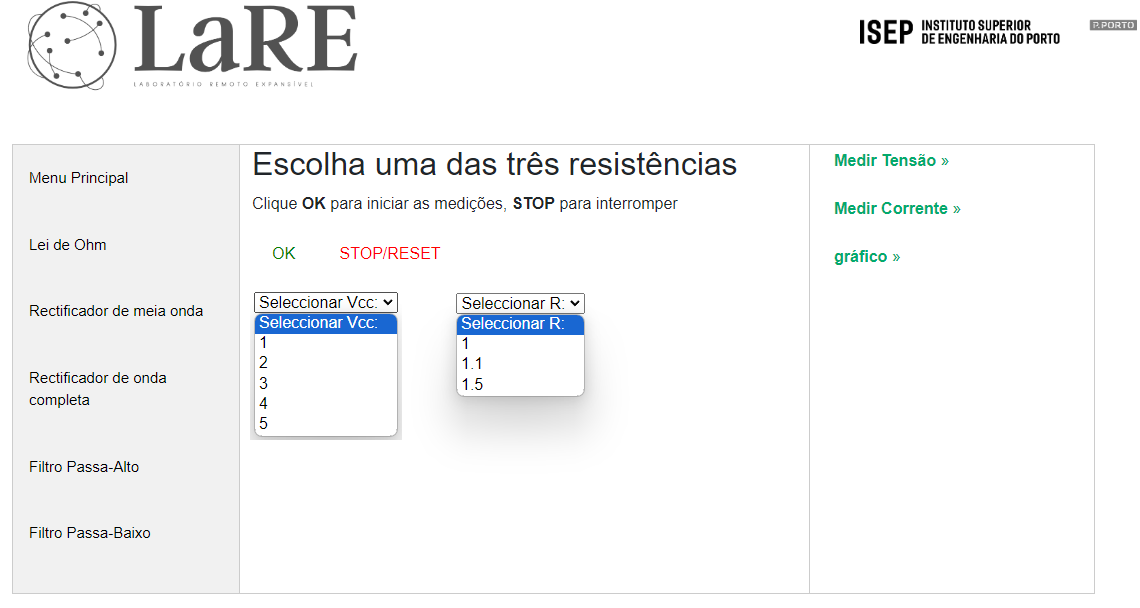
\includegraphics[width=6.3cm]{figures/ohm_escolha.png} }}%
		\qquad
		\subfloat[\centering Opção 2\label{fig:Opção_2}]{{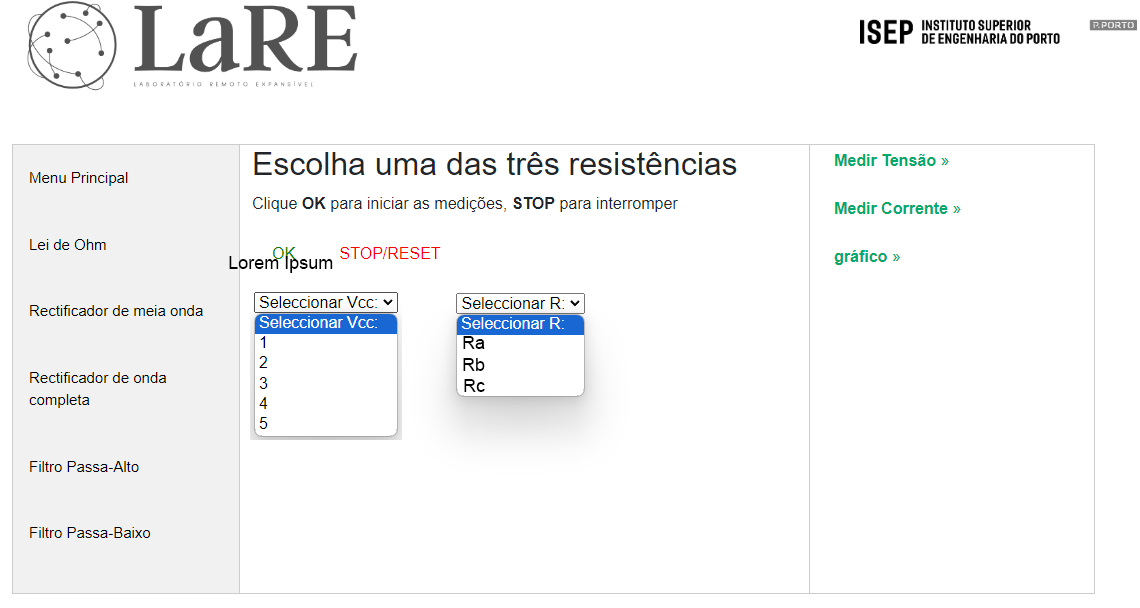
\includegraphics[width=6.3cm]{figures/ohm_escolha_abc.png} }}%
		\caption{Experiência Lei de \textit{Ohm}}%
		\label{fig:experienciaOHM}%
	\end{figure}

Dado que se optou pela liberdade de escolha aos utilizadores, a abordagem à implementação foi um desafio. (\textbf{se calhar retirava este parágrafo})

Para melhor descrever esta experiência e o seu funcionamento no que diz respeito ao \textit{software}, pode dividir-se a explicação em duas etapas: configuração inicial do \acrshort{virtualbench} e medição de tensão e corrente - \textbf{eventualmente três partes com o PI metido ao barulho}. 

A Figura \ref{fig:fluxohm} representa o fluxograma(??) completo do processo de execução da experiência. No entanto, para a primeira etapa, o foco será na comunicação entre a página \textit{ohm.html} e o ficheiro \textit{configVB.py}, representado na Figura \ref{fig:comohmconfigvb}.

\begin{figure}[hbtp]
	\centering
	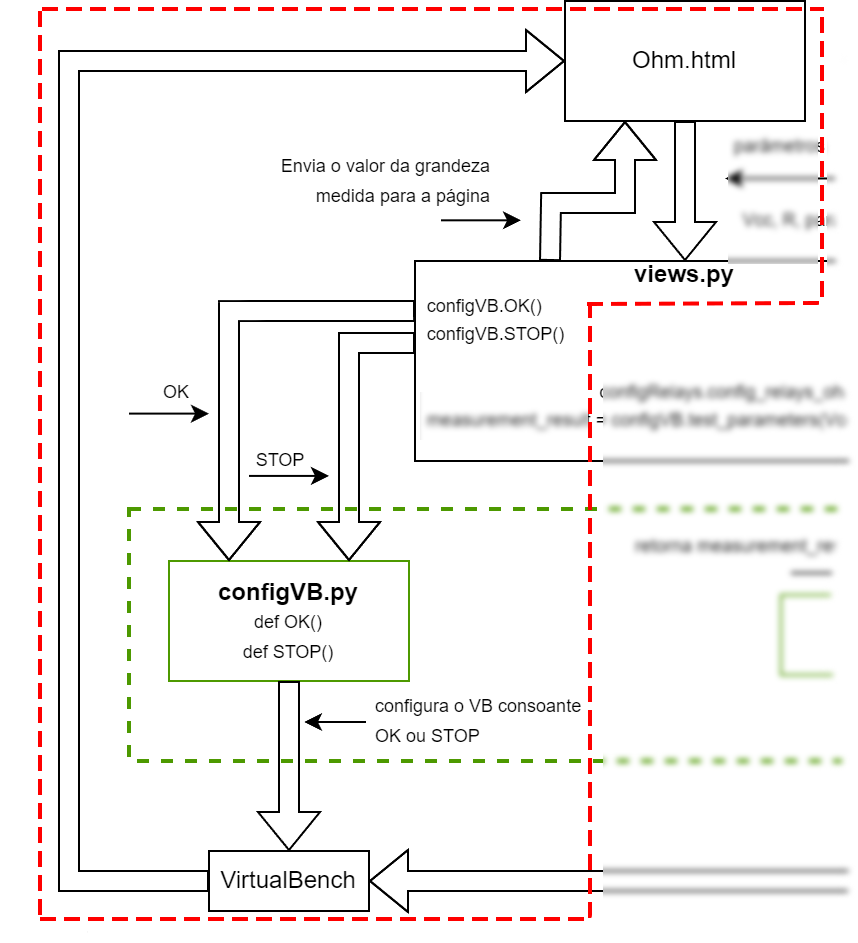
\includegraphics[width=0.6\textwidth]{figures/experiencia_ohm_diagrama.drawio.png}
	\caption{Comunicação \textit{ohm.html} e \textit{configVB.py}}
	\label{fig:comohmconfigvb}
\end{figure}

%FIQUEI AQUI - COMEÇAR POR DIZER QUE NESTA PARTE ENVOLVE 3 FICHEIROS, TALVEZ DE UMA FORMA MUITO RESUMIDA E DEPOIS PARTIR PARA UMA PARTE RIGOROSA

%EXPLICAR PORQUE SE COLOCOU UM BOTÃO DE OK E STOP/RESET, O PROMENOR DAS FONTES DE12v SEREM PRIMEIRO ACTIVADA AINDA NÃO ESTÁ EXPLICADA EM QQ LADO E FOI POR ISSO QUE SE OPTOU POR COLOCAR OS BOTÕES, AO FAZER RESET, OS ci E OS RELE´S DEIXAM DE ESTAR SOB TENSÃO.
%PORTNATO, O PASSO É, PRIMEIRO ACTIVAR IC E RELES, EFECTUAR MEDIÇÕES. NO FIM DA EXPERIENCIA AO CLICAR EM STOP A FONTE É DESLIGADA

%Entre estes dois ficheiros há envio/recepção de parâmetros.

Como se pode ver nas Figura \ref{fig:ohm_ctrl}, representadas na Secção \ref{sec:paginas}, a página \textit{ohm.html} é composta por um formulário que permite ao utilizador escolher os parâmetros $V_{CC}$ e R, assim como a medição a efectuar - corrente ou tensão e a construção do gráfico.

%\sout{O botão ``OK'' é responsável por habilitar os selectores de parâmetros, assim como habilitar a fonte de 25 do virtualbench. Enquanto que o botão ``STOP/RESET'' é responsável por interromper a experiência e desligar a fonte de alimentação.}

A verificação e detecção dos erros acontece quando o utilizador tenta seleccionar um dos parâmetros, antes de estes estarem habilitados, como exemplificado na Figura \ref{fig:erropagina}. 

\begin{figure}[hbtp]
	\centering
	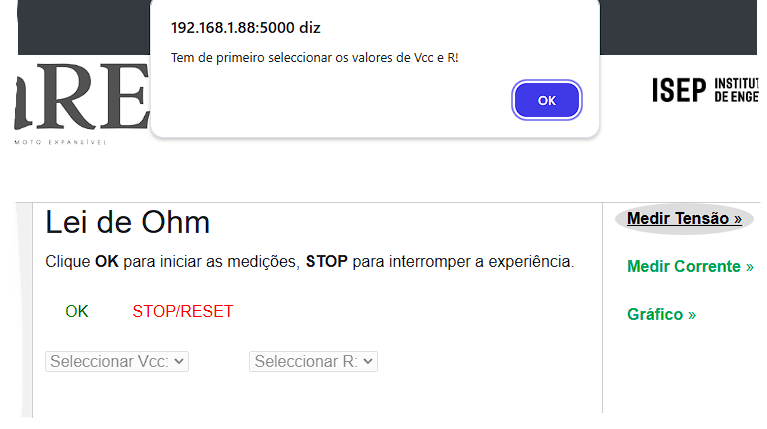
\includegraphics[width=0.7\textwidth]{figures/erro_pagina.png}
	\caption{Erro de selecção}
	\label{fig:erropagina}
\end{figure}

A Listagem \ref{lst:erro} mostra como o alerta está implementado, directamente na página \acrshort{html}.

\begin{center}
	\begin{minipage}{0.7\linewidth}
		\begin{lstlisting}[language=html, caption=Erro na página \textit{ohm.html}, label=lst:erro]
		(...)
        if (Vcc === "0" || Resistance === "0") {
          alert("Tem de primeiro seleccionar os valores de Vcc e R!");
          return;
        }
		(...)
	\end{lstlisting}
	\end{minipage}
\end{center}

No entanto, os parâmetros escolhidos só serão efectivamente enviados para o servidor \textit{Flask} - (\textit{views.py}) e a medição efectuada quando:
\begin{enumerate}
	\item Seleccionar o botão ``OK'' que habilita os selectores;
	\item Escolher ambos os parâmetros - $V_{CC}$ e R;
	\begin{enumerate}
		\item Clicar no link ``Medir tensão'' ou ``Medir corrente''.
	\end{enumerate}
\end{enumerate}

%Sequência: 
%1º passo:
%OK - habilita selectores na página HTML e envia o parâmetro para configurar a fonte de 25V, através do ficheiro configVB
%2º passo:
%Seleccionar os parâmetros $V_{CC}$ e R
%3º passo:
%Efectuar medição de tensão ou corrente, através do ficheiro configVB

\paragraph{Configuração inicial do VB} ~\\
Partindo da sequência anterior, o primerio passo (1.) é a habilitação dos selectores e a configuração da fonte de \SI{25}{\volt}. Pela análise da Figura \ref{fig:fluxohm}, os parâmetros são enviados da página \textit{ohm.html} para o \textit{script views.py}, da forma como indica a Listagem \ref{lst:exemploenvioparametros}.
%, é feita da forma apresentada na Listagem \ref{lst:exemploenvioparametros}:

\begin{center}
	\begin{minipage}{0.7\linewidth}
		\begin{lstlisting}[language=Html,escapechar=|, caption=Envio de parâmetros da página \textit{ohm.html} para o \textit{script views.py}, label=lst:exemploenvioparametros]
		(...)
		const booleanParameter = true; |\label{line:trueparameter}|
		const url = 
		`/config_VirtualBench?habilitar_parameter=${booleanParameter.toString()}`
		(...)
	\end{lstlisting}
	\end{minipage}
\end{center}

Do lado do servidor - \textit{script views.py} - os parâmetros são recebidos da forma como se pode ver na Listagem \ref{lst:exemplorecepcaoparametros}:
\begin{center}
	\begin{minipage}{1\linewidth}
		\begin{lstlisting}[language=Python,escapechar=|, caption=Recepção dos parâmetros no \textit{script views.py} enviados da página \textit{ohm.html}, label=lst:exemplorecepcaoparametros]
			(...)
			@views.route('/config_VirtualBench', methods=['GET', 'POST'])
			@login_required
			def config_VirtualBench():
				try:
					Vcc = request.args.get('Vcc', 0, int)|\label{line:vccref}|
					Resistance = request.args.get('R', 0, int)
					measure_parameter = request.args.get('parameter', 0, str)|\label{line:measureref}|
					configOK = request.args.get('habilitar_parameter', 0, bool)
					configSTOP = request.args.get('desabilitar_parameter', 0, bool)|\label{line:stopref}|
			(...)
		\end{lstlisting}
	\end{minipage}
\end{center}

Na função \textit{config\_VirtualBench()}, caso os parâmetros não existam, ou se não forem recebidos, linhas \ref{line:vccref} a \ref{line:stopref}, será retornado o valor ``0''.

A Figura \ref{fig:passagemparametros} mostra um exemplo dos valores que o ficheiro \textit{views.py} recebe, quando se carregar no botão ``OK'':
\begin{figure}[hbtp]
	\centering
	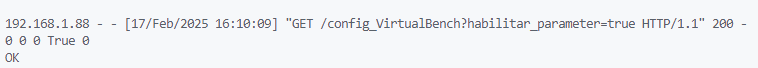
\includegraphics[width=1\textwidth]{figures/exemplo_dados_Ohm.png}
	\caption{Exemplo: passagem de parâmetros}
	\label{fig:passagemparametros}
\end{figure}

O único parâmetro que é passado, é respeitante ao botão ``OK'', que foi definido como \textit{``True''}, representado na Linha \ref{line:trueparameter}, da Listagem \ref{lst:exemploenvioparametros}.

Através da Listagem \ref{lst:recepcaoparametros} pode ver-se que, quando é recebido o parâmetro ``OK'', é chamada a função \textit{OK()}, Linha \ref{line:configOK}, do \textit{script} \textit{configVB.py}. O procedimento é em tudo idêntico quando é seleccionado o parâmetro ``STOP''.

\begin{minipage}{0.9\linewidth}
	\begin{lstlisting}[language=python, escapechar=|, caption=Teste do parâmetro ``OK'' (\ldots e ``STOP'') no ficheiro \textit{views.py}, label=lst:recepcaoparametros]
	(...)
	configOK = request.args.get('habilitar_parameter', None, bool)
	(...)
	if configOK == True:
        configVB.OK() |\label{line:configOK}|  
    elif configSTOP == True:
        configVB.STOP()	
	(...)
	\end{lstlisting}
\end{minipage}

O ficheiro \textit{configVB.py} é responsável pela configuração do \acrshort{virtualbench} - E NÃO SÓ - e pela construção do gráfico final. Além das supra-mencionadas inclui ainda as seguintes funções:
\begin{itemize}
	\item \textit{OK()};
	\item \textit{STOP()};
	\item \textit{test\_parameters(Vcc:int, R:int, measure\_parameter:str)};
	\item \textit{plot\_graphic(current\_measurements, voltage\_measurements)}.
\end{itemize}

Como já referido anteriormente, a função ``OK()'' é responsável por activar a fonte de alimentação de \SI{25}{\volt} do \acrshort{virtualbench}, configurá-la para \SI{12}{\volt} e habilitar os selectores dos parâmetros $V_{CC}$ e R. 

% referencia fontesalimentacao Coa fonte de 12V que vai alimentar os integrados e, através do LM317, a fonte de 5V. 

A função ``STOP()'' desactiva e liberta todas as saídas do \acrshort{virtualbench}, assim como os instrumentos e o próprio \acrshort{virtualbench}. Os selectores dos parâmetros $V_{CC}$ e R também são desabilitados.

Na Listagem \ref{lst:exemploOKPS} e Listagem \ref{lst:exemploSTOPPS} pode ver-se um exemplo de configuração da fonte de alimentação e do \textit{RESET}, respectivamente. 

\begin{minipage}{0.9\linewidth}
	\begin{lstlisting}[language=python, escapechar=|, caption=Exemplo de configuração: fonte de alimentação - OK, label=lst:exemploOKPS]
		(...)
		channel = "ps/+25V"
		voltage_level = 12.0
		current_limit = 0.5 
		ps.enable_all_outputs(True)
		ps.configure_voltage_output(channel, voltage_level, current_limit)
		(...)
	\end{lstlisting}
\end{minipage}

\begin{minipage}{0.9\linewidth}
	\begin{lstlisting}[language=python, escapechar=|, caption=Exemplo de configuração: fonte de alimentação - STOP, label=lst:exemploSTOPPS]
		(...)
		if all([ps, dmm, virtualbench]):
		   	ps.enable_all_outputs(False)
        	ps.release()
        	dmm.release()
        	virtualbench.release()
		(...)
	\end{lstlisting}
\end{minipage}

Analisado procedimento de configuração inicial do \acrshort{virtualbench}, o próximo passo (2.) é a medição de tensão e corrente e envio/recepção dos respectivos parâmetros.

\paragraph{Medição da tensão e corrente} ~\\
Na Listagem \ref{lst:exemploenvioparametros} é possível observar como o parâmetro é enviado para o ficheiro \textit{views.py}. No entanto, nesta etapa, são transmitidos três parâmetros: $V_{CC}$, R e o tipo de medição a realizar — corrente ou tensão. O método de envio desses parâmetros é idêntico ao utilizado para um único parâmetro, conforme ilustrado na Listagem \ref{lst:envioparmedidas}.

\begin{minipage}{0.9\linewidth}
	\begin{lstlisting}[language=html, escapechar=|, caption=Envio de parâmetros da página \textit{ohm.html} para \textit{views.py}, label=lst:envioparmedidas]
		(...)
		const parameter = this.dataset.parameter;
		(...)
		const url = `/config_VirtualBench?parameter=${parameter}&Vcc=${Vcc}&R=${Resistance}`;
        fetch(url)
		(...)
	\end{lstlisting}
\end{minipage}

Na Listagem \ref{lst:exemplorecepcaoparametros}, Linhas \ref{line:vccref} a \ref{line:measureref} é possível observar como os parâmetros são recebidos no ficheiro \textit{views.py}.

Após o teste aos parâmetros recebidos, o procedimento pode ser descrito da seguinte forma:
\begin{itemize}
	\item Configurar os relés;
	\item Configurar o \acrshort{virtualbench} e efectuar a medição;
	\item Desligar todos os relés.
\end{itemize}

\textbf{ATENÇÃO - Não esquecer de explicar a rebienga do store e get, nestas funções e o porquê}

\vspace{1cm}

O procedimento pode ser visto na Listagem \ref{lst:procedimentomedicao}, sendo que a Linha \ref{line:configrelays} é responsável por activar os relés, a Linha \ref{line:measureresult} configura o \acrshort{virtualbench}e efectua a medição da grandeza e a Linha \ref{line:stoprelays} desactiva os relés.

\begin{minipage}{0.9\linewidth}
	\begin{lstlisting}[language=python, escapechar=|, caption=Procedimento de medição, label=lst:procedimentomedicao]
		(...)
		configRelays.config_relays_ohm(Resistance, measure_parameter) |\label{line:configrelays}|
		time.sleep(2)
		measurement_result = configVB.test_parameters(Vcc, Resistance, measure_parameter) |\label{line:measureresult}|
		configRelays.config_relays_ohm(0, measure_parameter) |\label{line:stoprelays}|
		(...)
	\end{lstlisting}
\end{minipage}


A configuração dos relés é realizada no ficheiro 

ANALISOU-SE ANTERIORMENTE O PROCEDIMENTO DE OK E STOP-RESET. VAMOS AGORA PARA O ENVIO DOS RESTANTES PARAMENTROS E MEDIÇÕES

!!!!!!!!!! FIQUEI AQUI !!!!!!!!!!
REFERIR, TALVEZ A FONTE DO FLASK, RESPEITANTE AO REQUEST.ARGS

O envio dos restantes parâmetros, $V_{CC}$, R, medição de corrente (I) ou tensão (U) é feito de forma idêntica.

Quando se trata de enviar o resultado das medições para a página \textit{ohm.html}, a comunicação é feita da forma como se pode ver nas Listagens \ref{lst:envioresultados} e \ref{lst:recepcaoresultados}:
\begin{center}
	\begin{minipage}{0.7\linewidth}
		\begin{lstlisting}[language=python, caption=Envio de resultados do servidor (\textit{views.py}) para a página \textit{ohm.html}, label=lst:envioresultados]
			(...)
			return jsonify({'measurement_result': measurement_result})
			(...)
	\end{lstlisting}
	\end{minipage}
\end{center}

\begin{center}
	\begin{minipage}{0.7\linewidth}
		\begin{lstlisting}[language=html, caption=Recepção de resultados na página \textit{ohm.html}, label=lst:recepcaoresultados]
			(...)
			fetch(url)
			.then((response) => response.json())
		.then((data) => {
		  document.getElementById("current-measure").innerHTML =
			data.measurement_result + " mA";
			(...)
			\end{lstlisting}
	\end{minipage}
\end{center}

\subsubsection{O \textit{script configVB.py}}
\textbf{Este script poderá eventualmente ficar enquadrado numa secção a criar, denominada ``Descrição dos scripts'' ou então, na descrição da experiência lei de ohm.}

\hrule
\hrule

Como se pode ver na Figura , os selectores estão desabilitados e os relés nao estão alimentados porque isso é feito através da fonte do VB e do LM317

Já se viu (\textbf{refirerir a secção}) que na experiência da Lei de \textit{Ohm}, o utilizador selecciona os valores da tensão e resistência através de um formulário, representado na página \textit{ohm.html} da forma como se pode ver na Listagem \ref{lst:formularioescolha}.

\begin{center}
	\begin{minipage}{0.7\linewidth}
		\begin{lstlisting}[language=html, caption=Formulário de escolha na página \textit{ohm.html},label=lst:formularioescolha]
			(...)
			<div style="display: inline-block; width: 200px">
      <select id="selectVcc" disabled>
        <option value="0">Seleccionar V<sub>cc</sub>:</option>
        <option value="1">1</option>
        <option value="2">2</option>
        <option value="3">3</option>
        <option value="4">4</option>
        <option value="5">5</option>
      </select>
    </div>

    <div style="display: inline-block; width: 200px">
      <select id="selectR" disabled>
        <option value="0">Seleccionar R:</option>
        <option value="1">1</option>
        <option value="2">1.1</option>
        <option value="3">1.5</option>
      </select>
			(...)
	\end{lstlisting}
	\end{minipage}
\end{center}

No entanto, optou-se por adicionar à página \textit{ohm.html} um botão ``OK'' que, ao ser seleccionado, activa os selectores e envia os parâmetros para o servidor. O \textit{script} \textit{configVB.py} é chamado no \textit{script views.py}, consoante o valor do parâmetro recebido. A Figura  representa o diagrama de blocos do \textit{script}.

explicar porque se optou por colocar o botão ``OK'' e não enviar os parâmetros automaticamente, e só efectuar a medição quando se clicar no link medir.

Aqui vai ter de seexplicar porque se activa o OK. O Ok activa, antes de mais, a fonte de 12V que vai alimentar os integrados e, através do LM317, a fonte de 5V. 

Só depois os formulários são activos, permite seleccionar os valores e só depois é que o uti.lizador pode clicar no link medir.
Isto permite que o utilizador tenha mais controlo sobre a experiência.

Explicar porque é chamado o \textit{script configVB.py} e o que faz cada funlção
OK faz....
STOP faz....

Explicar porque os selectores estão desabilitados, foi o critério utilizado para realizar a configuração inicial do VB. Assim, quando dse carrega no "OK", habilitam-se os selectores e ao mesmo tempo, enviam-se os parâmetros para o servidor, de forma a configurar o VB. Que tipo de configuração se faz? Activa-se a fonte de 12V - colocar exemplo do programa e referenciar esquema de ligações - e alimentam-se os integrados de 12V e 5V - colocar ou referenciar o esquema

Na Secção anterior descreveu-se o processo de comunicação entre a página \textit{ohm.html} e o \textit{script views.py} (servidor).

O primeiro a ser chamado, como pode ser vist
\begin{figure}[hbtp]
	\centering
	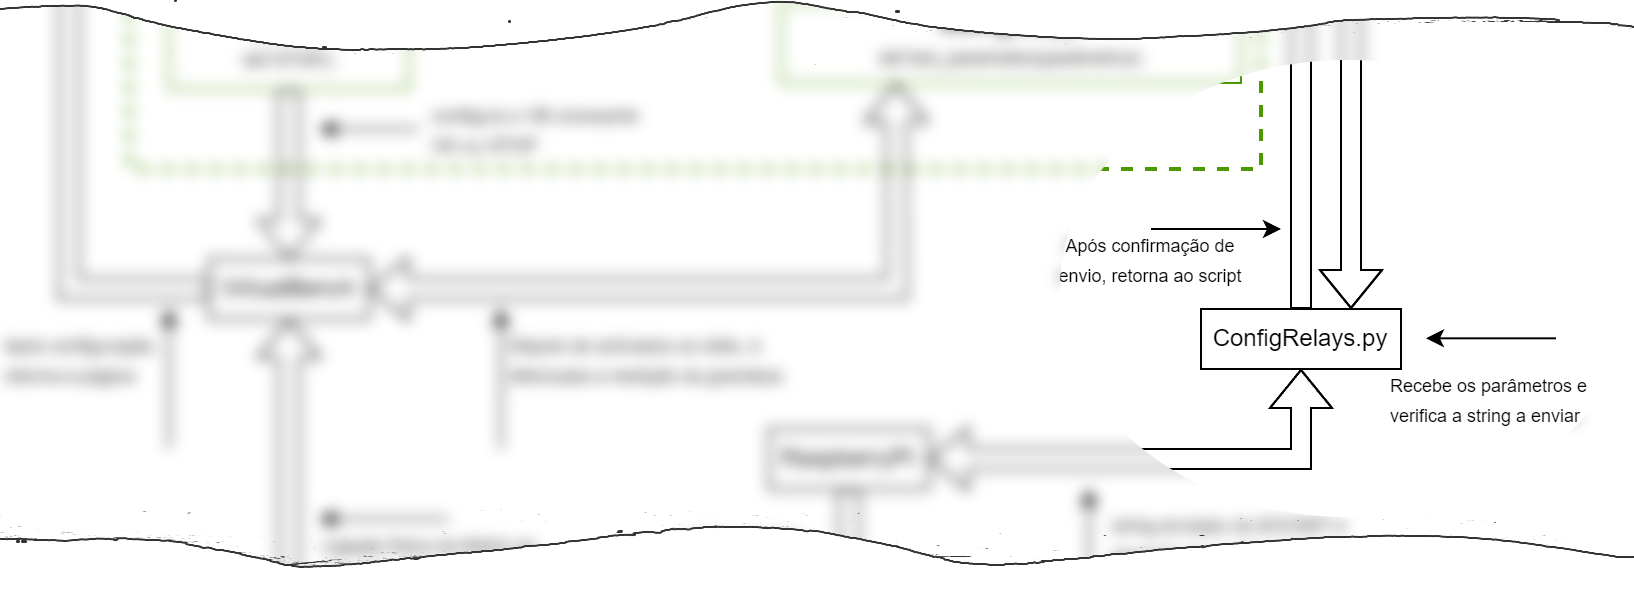
\includegraphics[width=1\textwidth]{figures/ohm_diagramaCUTRelay.drawio.png}
	\caption{\textit{Script configRelays.py}}
	\label{fig:cutconfigRelays}
\end{figure}

\section{qualquer coisa que ainda não sei o quê}

Após análise e estudo da informação presente no \textit{site} do \textit{Flask} e nos tutoriais mencionados em cima, definiu-se e implementou-se a página de autenticação no ficheiro \textit{auth.py}, tal como pode ser visto na Figura \ref{fig:paglogin}:

\begin{figure}[hbtp]
	\centering
	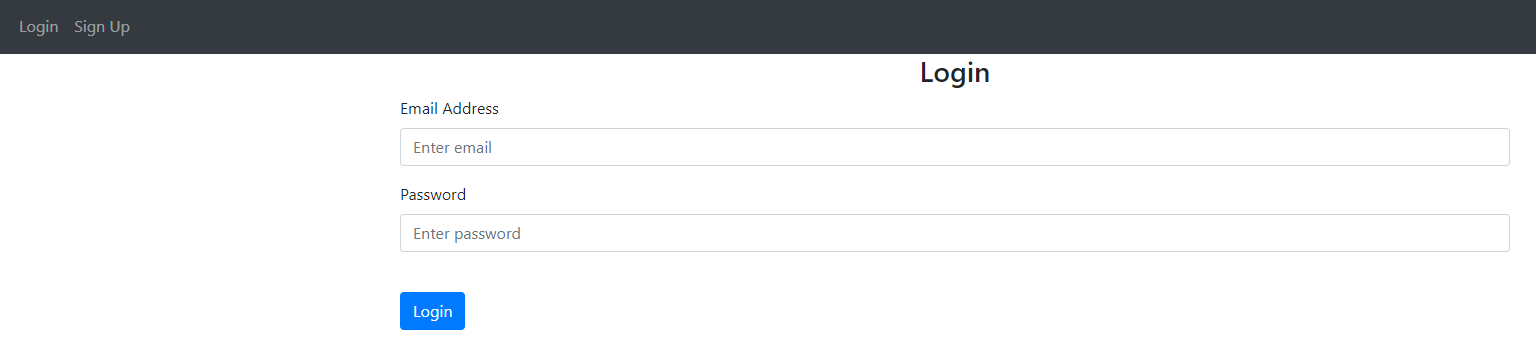
\includegraphics[width=1\textwidth]{figures/login.png}
	\caption{Página de \textit{login}}
	\label{fig:paglogin}
\end{figure}

\begin{figure}[hbtp]
	\centering
	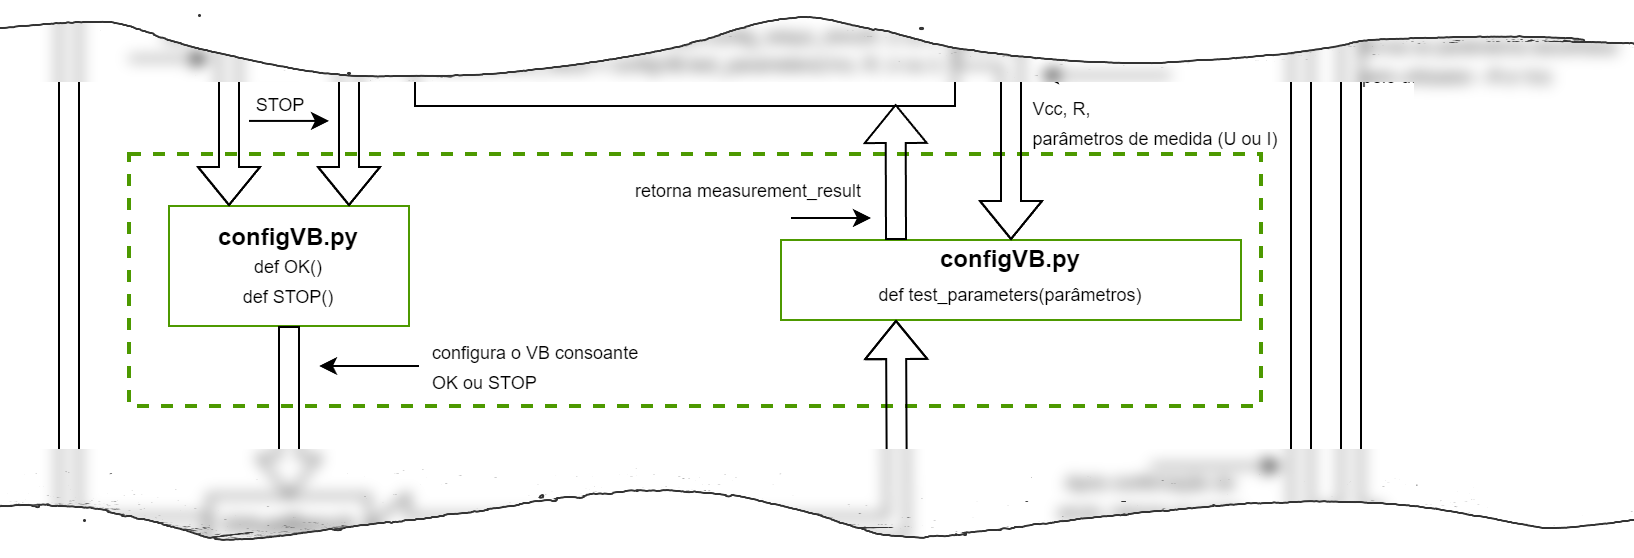
\includegraphics[width=1\textwidth]{figures/ohm_diagramaCUT.drawio.png}
	\caption{caralho}
	\label{fig:diagramaCUT}
\end{figure}

Um exemplo de como foi implementada a função \textit{login}() está representada na Listagem \ref{lst:exemplologin} e a rota está definida para a página \textit{/login}, como apresentado na mesma Figura, linha 17.

Os dados de \textit{login} e registo são guardados na directoria \textit{instance}, ficheiro \textit{database.db}.

Além da rota definida para o \textit{login}, as outras rotas definidas no ficheiro \textit{auth.py} foram as \textit{sign-up} e \textit{logout}. A estrutura base da função \textit{login}, representada na Listagem \ref{lst:exemplologin}, é idêntica para as restantes, sendo que ``/\textit{login''} representa a rota especificada, dentro da função há o código especifico inerentes a cada função e o \textit{return render\_template} indica qual a página a ser renderizada.

A juntar às páginas que compõem a estrutura base do \textit{site}, representadas na Figura \ref{fig:estruturapastas}, há ainda a juntar as páginas que permitem ao utilizador interagir com as experiências do \acrshort{lare}. Neste caso, serão cinco páginas, correspondentes aos 5 circuitos definidos na Secção \ref{sec:solucaoproposta}.

O menu de escolha foi retirado do \textit{site} \href{https://www.w3schools.com/howto/howto_js_vertical_tabs.asp}{\textit{w3schools}} e modificado de acordo com as necessidades do projecto, tal como pode ser visto na Figura \ref{fig:pagmenu}.

As páginas referentes às experiências seguem a mesma estrutura de menus.

\sout{Uma das partes mais cruciais e que levantou mais dificuldades foi a comunicação e o envio de parâmetros entre as páginas \acrshort{html} e o \textit{Flask}.}

\hrule
fim
\hrule

Na secção seguinte explica-se a solução encontrada.
